\documentclass[
    aps,
    pra,
    reprint,
    superscriptaddress,
    nofootinbib
]{revtex4-2}

\usepackage{amsmath}
\usepackage{amssymb}
\usepackage{amsthm}
\usepackage{mathtools}
\usepackage{bm}
\usepackage{braket}
\usepackage{booktabs}
\usepackage{tabularx}
\usepackage{array}

\usepackage{graphicx}
\usepackage{tikz}

\usetikzlibrary{
    arrows.meta,
    positioning,
    matrix,
    fit,
    decorations.pathreplacing
}

\usepackage[T1]{fontenc}
\usepackage{lmodern}
\usepackage{microtype}
\usepackage{xcolor}
\definecolor{linkblue}{RGB}{35,55,115}

\usepackage[
    colorlinks=true,
    allcolors=linkblue
]{hyperref}

\setlength{\parindent}{1em}
\setlength{\parskip}{0pt}

\theoremstyle{definition}
\newtheorem{definition}{Definition}[section]
\newtheorem{example}{Example}[section]

\theoremstyle{plain}
\newtheorem{theorem}{Theorem}[section]
\newtheorem{lemma}[theorem]{Lemma}
\newtheorem{proposition}[theorem]{Proposition}

\begin{document}
\title{A Tensor Formulation of the Choi--Jamio{\l}kowski Isomorphism for
Quantum and Hybrid Networks}
\author{Joaquim Regis}
\email{rgs.joaquim@gmail.com}
\affiliation{IRIF, Université Paris Cité, CNRS, Paris, France}
\affiliation{Department of Mathematics, University of York, York, United Kingdom}
\begin{abstract}
We develop a unified operator and tensor framework for the local factors of
classical, quantum, and hybrid Bayesian networks. Finite probability
distributions are represented as diagonal density operators, while
conditional probability distributions give rise to positive conditional
operators that, through the Choi--Jamio{\l}kowski isomorphism, coincide with
the Choi operators of the quantum channels induced by the corresponding
stochastic maps. This identifies classical conditional probabilities as a
special class of quantum channels and places classical and quantum nodes of
a directed acyclic graph within a common positive-operator formalism.
Representing these operators as tensors in fixed orthonormal bases, we
show that channel action reduces to a contraction over the input indices,
providing a unified computational language for network composition.
Classical Bayesian-network factor multiplication, quantum channel
composition, and the interaction of state preparation and measurement in
hybrid networks all emerge as instances of the same tensor-contraction
rules.
\end{abstract}

\maketitle


\section{Introduction}

Bayesian networks describe probabilistic systems by means of directed
acyclic graphs, with a local probability distribution associated with each
node, conditioned on its parents
\cite[Sec.~11.2.3]{Darwiche2008}. When quantum systems are included in the
network, their local transformations are described by quantum channels
rather than by conditional probability distributions. The starting point
of this work is to ask whether these classical and quantum factors can be
represented in a common operator language and combined within the same
component formalism.

A finite probability distribution can be represented by a density operator
that is diagonal in the basis indexed by its possible values. Applying the
same construction to a conditional distribution
$p_{\mathsf{X}|\mathsf{Y}}$ gives a positive operator
$\rho_{\mathsf{X}|\mathsf{Y}}$ satisfying
\begin{equation}
    \mathrm{Tr}_{\mathcal{X}}
    \left(
        \rho_{\mathsf{X}|\mathsf{Y}}
    \right)
    =
    \mathrm{Id}_{\mathcal{Y}}.
\end{equation}
This conditional operator is not merely another way of recording the
conditional probabilities. Its positivity and normalization are precisely
the conditions required of the Choi operator of a quantum channel. Through
the Choi--Jamio{\l}kowski isomorphism,
$\rho_{\mathsf{X}|\mathsf{Y}}$ is the Choi operator of the channel induced
by the stochastic map associated with
$p_{\mathsf{X}|\mathsf{Y}}$. The stochastic maps defined by classical
conditional distributions therefore embed into quantum channels.

This observation gives a common representation of the local factors
associated with the nodes of a directed acyclic graph. A root factor is
represented by a density operator, a classical conditional factor by a
diagonal Choi operator, and a quantum conditional factor by the Choi
operator of a quantum channel. All these local factors are positive
operators, while the distinction between the classical and quantum cases
is expressed by their structure and normalization. This point of view is
related to the conditional-state formalism of Leifer and Spekkens
\cite{LeiferSpekkens2013} and to the Q-factor framework of Di Guardia,
Ehrhard, and Faggian~\cite{DiGuardiaEhrhardFaggian2026}.

Representing all local factors by operators leaves the question of how to
combine them. If $J(\Phi)$ is the Choi operator of a channel
$\Phi:L(\mathcal{Y})\to L(\mathcal{X})$, its action is
\begin{equation}
    \Phi(A)
    =
    \mathrm{Tr}_{\mathcal{Y}}
    \left(
        J(\Phi)
        \left(
            \mathrm{Id}_{\mathcal{X}}
            \otimes
            A^{T}
        \right)
    \right)
\end{equation}
\cite[Eq.~(2.66)]{Watrous2018}. Thus, the input is transposed, lifted to
the space of the Choi operator, multiplied by that operator, and finally
removed by a partial trace. For a single channel these operations are
direct, but when several channels are composed the registers involved in
each step become less apparent.

We therefore write the operators as tensors in fixed orthonormal bases.
The indices identify the registers to which the components belong, and the
action of a Choi operator is expressed directly by contracting its input
indices. The same description applies to channel composition: the indices
associated with an intermediate quantum register are contracted between
the corresponding channel factors. 
The same component notation can be used for classical and hybrid networks,
although the operations in the two cases are not identical. For diagonal
operators, factor multiplication reduces to the pointwise product used in
classical Bayesian networks. In a hybrid network, classically controlled
state preparations, quantum channel factors, and destructive measurements
are combined by contracting the intermediate quantum indices. The emphasis
of this paper is therefore on the representation and composition of local
classical and quantum factors, rather than on Bayesian inference.

Sections~\ref{sec:preliminaries}--\ref{sec:basic-quantum-information}
introduce the notation and mathematical background used in the paper.
Section~\ref{sec:classical-probability-operator} establishes the connection
between conditional distributions, conditional operators, and the quantum
channels induced by stochastic maps.
Section~\ref{sec:quantum-bayesian-networks} develops the tensor formulation
for classical Bayesian networks, quantum channel networks, and hybrid
classical--quantum networks.

\section{Preliminaries and Notation}
\label{sec:preliminaries}

All vector spaces considered below are finite-dimensional complex Euclidean
spaces. We follow the notation and conventions of
Watrous~\cite[Secs.~1.1.1--1.1.2 and 1.2.1]{Watrous2018}, with minor
adaptations for consistency with the tensor notation used in this paper.
This section fixes the notation needed for linear operators, maps on
operator spaces, and probability vectors.

\subsection{Complex Euclidean spaces}

An \emph{alphabet} is a finite, nonempty set whose elements are called
symbols. Alphabets are denoted by capital Greek letters such as $\Sigma$ and
$\Gamma$. For an alphabet $\Sigma$, define
\begin{equation}
    \mathbb{C}^{\Sigma}
    =
    \left\{u:\Sigma\to\mathbb{C}\right\}.
\end{equation}
Equipped with pointwise addition and scalar multiplication and with the
standard inner product, $\mathbb{C}^{\Sigma}$ is a complex Euclidean space
of dimension $\lvert\Sigma\rvert$.
Complex Euclidean spaces are denoted by script letters such as
$\mathcal{X}$, $\mathcal{Y}$, and $\mathcal{Z}$. We denote the standard
orthonormal basis of $\mathbb{C}^{\Sigma}$ by
$\{e_a:a\in\Sigma\}$.


\subsection{Linear operators}

For complex Euclidean spaces $\mathcal{X}$ and $\mathcal{Y}$, the space of
linear operators from $\mathcal{X}$ to $\mathcal{Y}$ is denoted
\begin{equation}
    L(\mathcal{X},\mathcal{Y})
    =
    \left\{A:\mathcal{X}\to\mathcal{Y}:A\ \text{is linear}\right\}.
\end{equation} We write $L(\mathcal{X})=L(\mathcal{X},\mathcal{X})$, and denote the identity operator on $\mathcal{X}$ by $\mathrm{Id}_{\mathcal{X}}$. Let $\mathcal{X}=\mathbb{C}^{\Sigma}$ and
$\mathcal{Y}=\mathbb{C}^{\Gamma}$. 
For $a\in\Gamma$ and $b\in\Sigma$, the matrix unit
$E_{a,b}\in L(\mathcal{X},\mathcal{Y})$ is defined by
\begin{equation}
    E_{a,b}(c,d)=
    \begin{cases}
        1, & (c,d)=(a,b),\\
        0, & \text{otherwise}.
    \end{cases}
    \qquad c\in\Gamma,\quad d\in\Sigma.
\end{equation} The collection $\{E_{a,b}:a\in\Gamma,\ b\in\Sigma\}$ is the standard basis of $L(\mathcal{X},\mathcal{Y})$.

For $A\in L(\mathcal{X},\mathcal{Y})$, the transpose relative to the
standard bases is the operator $A^{T}\in L(\mathcal{Y},\mathcal{X})$
defined by
\begin{equation}
    A^{T}(b,a)=A(a,b),
    \qquad a\in\Gamma,\quad b\in\Sigma.
\end{equation}

An operator
$H\in L(\mathcal{X})$ is \emph{Hermitian} when $H=H^\dagger$.
The trace of $X\in L(\mathcal{X})$ is
\begin{equation}
    \mathrm{Tr}(X)=\sum_{a\in\Sigma}X(a,a),
    \qquad \mathcal{X}=\mathbb{C}^{\Sigma}.
\end{equation}

\subsubsection{Positive, density, and diagonal operators}

\begin{enumerate}
    \item \emph{Positive semidefinite operators.}
    An operator $P\in L(\mathcal{X})$ is positive semidefinite if
    $P=A^\dagger A$ for some $A\in L(\mathcal{X})$. We denote the cone of
    positive semidefinite operators by
    \begin{equation}
        \mathrm{Pos}(\mathcal{X})
        =
        \left\{A^\dagger A:A\in L(\mathcal{X})\right\}.
    \end{equation}
    Equivalently, $P$ is positive semidefinite if and only if it is Hermitian
    and all its eigenvalues are nonnegative.

    \item \emph{Density operators.}
    A density operator is a positive semidefinite operator of trace one. The
    set of density operators on $\mathcal{X}$ is
    \begin{equation}
        D(\mathcal{X})
        =
        \left\{\rho\in\mathrm{Pos}(\mathcal{X}):
        \mathrm{Tr}(\rho)=1\right\}.
    \end{equation}

    \item \emph{Diagonal operators.}
    An operator $X\in L(\mathbb{C}^{\Sigma})$ is diagonal if $X(a,b)=0$
    whenever $a\neq b$.
\end{enumerate}

\subsection{Linear maps on operator spaces}

For complex Euclidean spaces $\mathcal{X}$ and $\mathcal{Y}$, let
\begin{equation}
    T(\mathcal{X},\mathcal{Y})
    =
    L\bigl(L(\mathcal{X}),L(\mathcal{Y})\bigr)
\end{equation}
denote the vector space of linear maps
$\Phi:L(\mathcal{X})\to L(\mathcal{Y})$. We denote the identity map on
$L(\mathcal{X})$ by $\mathrm{Id}_{L(\mathcal{X})}$. Upon identifying
$L(\mathbb{C})$ with $\mathbb{C}$, the trace is an element of
\begin{equation}
    \mathrm{Tr}\in T(\mathcal{X},\mathbb{C}).
\end{equation}

A map $\Phi\in T(\mathcal{X},\mathcal{Y})$ is \emph{positive} if
\begin{equation}
    \Phi(P)\in\mathrm{Pos}(\mathcal{Y})
    \qquad\text{for every }P\in\mathrm{Pos}(\mathcal{X}).
\end{equation}
It is \emph{trace-preserving} if
\begin{equation}
    \mathrm{Tr}\bigl(\Phi(X)\bigr)=\mathrm{Tr}(X)
    \qquad\text{for every }X\in L(\mathcal{X}).
\end{equation}


\subsection{Probability vectors}

For an alphabet $\Sigma$, a vector $p\in\mathbb{R}^{\Sigma}$ is a
\emph{probability vector} if
\begin{equation}
    p(a)\geq 0\quad\text{for every }a\in\Sigma,
    \qquad
    \sum_{a\in\Sigma}p(a)=1.
\end{equation}
The set of all probability vectors on $\Sigma$ is denoted
$\mathcal{P}(\Sigma)$.

\section{Tensor products and contractions}
\label{sec:tensor-products}

Composite quantum systems, Choi operators, and the tensor contractions used
later all rely on the same finite-dimensional tensor-product structure. We
therefore fix the relevant conventions here, including the relation between
operators and tensors. The conventions for tensor products
and maps on operator spaces follow
Watrous~\cite[Secs.~1.1.1--1.1.2]{Watrous2018}.

\subsection{Tensor-product conventions}

Let $n$ be a positive integer and let
$\mathcal{X}_{k}=\mathbb{C}^{\Sigma_{k}}$ for
$k\in\{1,\ldots,n\}$. We identify
\begin{equation}
    \mathcal{X}_{1}\otimes\cdots\otimes\mathcal{X}_{n}
    =
    \mathbb{C}^{\Sigma_{1}\times\cdots\times\Sigma_{n}}.
\end{equation}
For vectors $u_k\in\mathcal{X}_k$, we write
$u_1\otimes\cdots\otimes u_n$ for their elementary tensor.

For $A\in L(\mathcal{X},\mathcal{Y})$ and
$B\in L(\mathcal{Z},\mathcal{W})$, their tensor product is the operator
\begin{equation}
    A\otimes B
    \in
    L(\mathcal{X}\otimes\mathcal{Z},
      \mathcal{Y}\otimes\mathcal{W})
\end{equation}
characterized by
\begin{equation}
    (A\otimes B)(u\otimes v)
    =
    Au\otimes Bv.
\end{equation}
The same notation is used for tensor products of more than two operators.

For $\Phi\in T(\mathcal{X},\mathcal{Y})$ and
$\Psi\in T(\mathcal{Z},\mathcal{W})$, their tensor product is the unique
linear map
\begin{equation}
    \Phi\otimes\Psi
    \in
    T(\mathcal{X}\otimes\mathcal{Z},
      \mathcal{Y}\otimes\mathcal{W})
\end{equation}
such that
\begin{equation}
    (\Phi\otimes\Psi)(X\otimes Z)
    =
    \Phi(X)\otimes\Psi(Z)
\end{equation}
for every $X\in L(\mathcal{X})$ and $Z\in L(\mathcal{Z})$.

\subsubsection{Completely positive maps}

A map $\Phi\in T(\mathcal{X},\mathcal{Y})$ is \emph{completely positive} if
\begin{equation}
    \Phi\otimes\mathrm{Id}_{L(\mathcal{Z})}
    \in
    T(\mathcal{X}\otimes\mathcal{Z},
      \mathcal{Y}\otimes\mathcal{Z})
\end{equation}
is positive for every complex Euclidean space $\mathcal{Z}$. The set of all
such maps is denoted $\mathrm{CP}(\mathcal{X},\mathcal{Y})$.

\subsubsection{Partial trace}

For complex Euclidean spaces $\mathcal{X}$ and $\mathcal{Y}$, the partial
trace over $\mathcal{X}$ is
\begin{equation}
    \mathrm{Tr}_{\mathcal{X}}
    :=
    \mathrm{Tr}\otimes\mathrm{Id}_{L(\mathcal{Y})}
    \in T(\mathcal{X}\otimes\mathcal{Y},\mathcal{Y}).
\end{equation}
It is characterized on elementary operators by
\begin{equation}
    \mathrm{Tr}_{\mathcal{X}}(A\otimes B)
    =
    \mathrm{Tr}(A)B,
    \qquad
    A\in L(\mathcal{X}),\quad B\in L(\mathcal{Y}).
\end{equation}
Similarly,
\begin{equation}
    \mathrm{Tr}_{\mathcal{Y}}
    :=
    \mathrm{Id}_{L(\mathcal{X})}\otimes\mathrm{Tr}
    \in T(\mathcal{X}\otimes\mathcal{Y},\mathcal{X}).
\end{equation}

\subsection{Tensors and contractions}
\label{subsec:tensors-contractions}

The tensor notation used later keeps track of the input and output indices
associated with each subsystem. We only recall the conventions needed
below; more detailed treatments are given by
Greub~\cite[Secs.~3.12--3.13]{Greub1978},
Wendl~\cite[Secs.~A.6--A.7, pp.~175--180]{Wendl2008Multilinear}, and
Dullemond and
Peeters~\cite[pp.~13 and 21--22]{DullemondPeeters2010}.

\begin{definition}
    Let $V_{1},\ldots,V_{m}$ and $W_{1},\ldots,W_{n}$ be
    finite-dimensional complex vector spaces. A tensor of type
    $(m,n)$ is an element
    \begin{equation}
        T\in
        (V_{1}\otimes\cdots\otimes V_{m})
        \otimes
        (W_{1}^{*}\otimes\cdots\otimes W_{n}^{*}).
    \end{equation}
    Its order is $m+n$. Given bases $\{e^{(a)}_{i_{a}}\}$ of $V_{a}$ and
    $\{f^{(b)}_{j_{b}}\}$ of $W_{b}$, with dual bases
    $\{f_{(b)}^{j_{b}}\}$, the components of $T$ are defined by
    \begin{equation}
        \begin{aligned}
        T={}&
        \sum_{\substack{i_{1},\ldots,i_{m}\\
                        j_{1},\ldots,j_{n}}}
        T^{i_{1}\cdots i_{m}}{}_{j_{1}\cdots j_{n}}
        \bigl(
            e^{(1)}_{i_{1}}\otimes\cdots\otimes e^{(m)}_{i_{m}}
        \bigr)\\
        &\otimes
        \bigl(
            f_{(1)}^{j_{1}}\otimes\cdots\otimes f_{(n)}^{j_{n}}
        \bigr).
        \end{aligned}
    \end{equation}
    The upper indices are contravariant and label the vector factors,
    whereas the lower indices are covariant and label the dual-vector
    factors.
\end{definition}

A contraction may pair only a contravariant index with a covariant index
referring to the same vector space
\cite[p.~22]{DullemondPeeters2010}. For example, if $V_{m}=W_{1}$ and the
corresponding bases agree, then
\begin{equation}
    S^{i_{1}\cdots i_{m-1}}{}_{j_{2}\cdots j_{n}}
    =
    T^{i_{1}\cdots i_{m-1}k}{}_{k j_{2}\cdots j_{n}}.
\end{equation}
The repeated index $k$ is summed over, while the remaining indices are
free. This is the Einstein summation convention, which we use unless a
different convention is stated explicitly.

For finite-dimensional complex vector spaces $V$ and $W$, there is a
canonical, basis-independent isomorphism
\cite[Sec.~1]{Conrad2006TensorMaps}
\begin{equation}
    L(V,W)\simeq W\otimes V^{*}
\end{equation}
under which every linear operator corresponds to a unique tensor, and
conversely~\cite[Sec.~1.28]{Greub1978}. This identification allows us to
regard an operator on
$\mathcal{X}_{1}\otimes\cdots\otimes\mathcal{X}_{r}$ as a tensor
carrying one upper and one lower index for each subsystem, as we will
exploit later.


\section{Quantum states, channels, and measurements}
\label{sec:basic-quantum-information}

We associate each register with a finite-dimensional complex Euclidean space.
Quantum states of the register are represented by density operators, while
transformations between registers are represented by quantum channels. We
also introduce the description of measurement outcomes that will be needed
for the classical--quantum networks considered later. Our conventions follow
Watrous~\cite[Secs.~2.1.1--2.1.2]{Watrous2018}.

\subsection{Registers and states}

\subsubsection{Registers and classical state sets}

\begin{definition}
    Registers are defined as follows:
    \begin{enumerate}
        \item every alphabet $\Sigma$ is a register;
        \item if $n$ is a positive integer and
        $\mathsf{Y}_1,\ldots,\mathsf{Y}_n$ are registers, then
        $\mathsf{X}=(\mathsf{Y}_1,\ldots,\mathsf{Y}_n)$ is a register.
    \end{enumerate}
\end{definition}

Registers of the first type are called \emph{simple}, whereas tuples of
registers are called \emph{compound}.

\begin{definition}
    The \emph{classical state set} of a register $\mathsf{X}$ is specified
    recursively:
    \begin{enumerate}
        \item if $\mathsf{X}=\Sigma$ is simple, its classical state set is
        $\Sigma$;
        \item if
        $\mathsf{X}=(\mathsf{Y}_1,\ldots,\mathsf{Y}_n)$ is compound and
        $\Sigma_k$ is the classical state set of $\mathsf{Y}_k$, then the
        classical state set of $\mathsf{X}$ is
        \begin{equation}
            \Sigma_1\times\cdots\times\Sigma_n.
        \end{equation}
    \end{enumerate}
\end{definition}

The elements of this set are the classical states of the register. In
particular, a classical state of a compound register specifies one classical
state for each of its constituent registers.

\subsubsection{Quantum states of registers}
\label{sec:quantum-state}

\begin{definition}
    If $\Sigma$ is the classical state set of a register $\mathsf{X}$, the
    complex Euclidean space associated with $\mathsf{X}$ is
    \begin{equation}
        \mathcal{X}=\mathbb{C}^{\Sigma}.
    \end{equation}
\end{definition}

Thus, if
$\mathsf{X}=(\mathsf{Y}_1,\ldots,\mathsf{Y}_n)$ and
$\mathcal{Y}_k=\mathbb{C}^{\Sigma_k}$ is the space associated with
$\mathsf{Y}_k$, the tensor-product convention fixed above gives
\begin{equation}
    \mathcal{X}
    =
    \mathbb{C}^{\Sigma_1\times\cdots\times\Sigma_n}
    =
    \mathcal{Y}_1\otimes\cdots\otimes\mathcal{Y}_n.
\end{equation}

\begin{definition}
    A \emph{quantum state} of a register $\mathsf{X}$ is a density operator
    $\rho\in D(\mathcal{X})$, where $\mathcal{X}$ is the complex Euclidean
    space associated with $\mathsf{X}$.
\end{definition}

\paragraph{Mixtures.}

The set $D(\mathcal{X})$ is convex. Thus, let $\Gamma$ be an alphabet, let
$\{\rho_a:a\in\Gamma\}\subseteq D(\mathcal{X})$, and let
$p\in\mathcal{P}(\Gamma)$. The operator
\begin{equation}
    \rho=\sum_{a\in\Gamma}p(a)\rho_a
\end{equation}
belongs to $D(\mathcal{X})$ and is called the mixture of the states
$\rho_a$ with probabilities $p(a)$.

\subsection{Quantum channels}

Quantum channels model transformations of register states. We use
the standard completely-positive, trace-preserving definition
\cite[Def.~2.13]{Watrous2018}.

\begin{definition}
    A \emph{quantum channel} from $\mathcal{X}$ to $\mathcal{Y}$ is a linear
    map
    \begin{equation}
        \Phi:L(\mathcal{X})\to L(\mathcal{Y})
        \label{eq:qc}
    \end{equation}
    that is completely positive and trace-preserving; equivalently,
    $\Phi\in\mathrm{CP}(\mathcal{X},\mathcal{Y})$ and
    \begin{equation}
        \mathrm{Tr}\bigl(\Phi(X)\bigr)=\mathrm{Tr}(X)
        \qquad\text{for every }X\in L(\mathcal{X}).
    \end{equation}
\end{definition}

A channel maps density operators to density operators. Consequently, if
$\mathsf{X}$ and $\mathsf{Y}$ have associated spaces $\mathcal{X}$ and
$\mathcal{Y}$, respectively, and $\mathsf{X}$ is prepared in the state
$\rho\in D(\mathcal{X})$, then the output state is
$\Phi(\rho)\in D(\mathcal{Y})$.

\subsection{Measurements}

The outcome statistics of a quantum measurement are described by a positive
operator-valued measure (POVM)~\cite[Def.~2.34]{Watrous2018}. In this paper,
measurements are used as destructive quantum-to-classical processes: only the
classical outcome is retained, while the postmeasurement quantum system is
discarded.

\begin{definition}
    A \emph{POVM} on $\mathcal{X}$ with outcome alphabet $\Sigma$ is a
    function
    \begin{equation}
        \mu:\Sigma\to\mathrm{Pos}(\mathcal{X})
    \end{equation}
    satisfying
    \begin{equation}
        \sum_{a\in\Sigma}\mu(a)=\mathrm{Id}_{\mathcal{X}}.
    \end{equation}
    If the measured state is $\rho\in D(\mathcal{X})$, the outcome
    distribution $p\in\mathcal{P}(\Sigma)$ is given by
    \begin{equation}
        p(a)=\mathrm{Tr}\bigl(\mu(a)\rho\bigr).
    \end{equation}
\end{definition}

The operator $\mu(a)$ is the POVM element associated with outcome $a$. We
may equivalently specify the measurement as a collection
$\{P_a:a\in\Sigma\}\subseteq\mathrm{Pos}(\mathcal{X})$, where
$P_a=\mu(a)$ and $\sum_{a\in\Sigma}P_a=\mathrm{Id}_{\mathcal{X}}$.


\section{Classical Probability in Operator Form}
\label{sec:classical-probability-operator}

Finite probability distributions can be represented by diagonal density
operators. We apply this representation to joint and conditional
distributions. The resulting conditional operator will then be identified,
through the Choi--Jamio{\l}kowski isomorphism, with the Choi operator of the
quantum channel induced by the corresponding stochastic map.

\subsection{Finite probability distributions}

Let $\mathsf{X}$ be a register with classical state set $\Sigma$. A
probabilistic state of $\mathsf{X}$ is a probability vector
$p_{\mathsf{X}}\in\mathcal{P}(\Sigma)$, where
$p_{\mathsf{X}}(x)$ is the probability that $\mathsf{X}$ is in the
classical state $x\in\Sigma$.

\paragraph{Joint and marginal distributions.}

Let $\mathsf{X}$ and $\mathsf{Y}$ be registers with classical state sets
$\Sigma$ and $\Gamma$, respectively. The compound register
$(\mathsf{X},\mathsf{Y})$ has classical state set
$\Sigma\times\Gamma$, so a joint probabilistic state is a probability vector
\begin{equation}
    p_{\mathsf{X},\mathsf{Y}}
    \in\mathcal{P}(\Sigma\times\Gamma).
\end{equation}
The value $p_{\mathsf{X},\mathsf{Y}}(x,y)$ is the probability associated
with the joint classical state $(x,y)$, and therefore
\begin{equation}
    \sum_{x\in\Sigma}\sum_{y\in\Gamma}
    p_{\mathsf{X},\mathsf{Y}}(x,y)=1.
\end{equation}
The corresponding marginal probabilistic states are
\begin{equation}
    p_{\mathsf{X}}(x)
    =
    \sum_{y\in\Gamma}p_{\mathsf{X},\mathsf{Y}}(x,y),
\end{equation}
for every $x\in\Sigma$, and
\begin{equation}
    p_{\mathsf{Y}}(y)
    =
    \sum_{x\in\Sigma}p_{\mathsf{X},\mathsf{Y}}(x,y),
\end{equation}
for every $y\in\Gamma$.

\paragraph{Conditional distributions.}

A conditional probabilistic state can be viewed as a function of the form
\begin{equation}
    p_{\mathsf{X}|\mathsf{Y}}:
    \Gamma\to\mathcal{P}(\Sigma).
\end{equation}
In other words, for each fixed $y\in\Gamma$, this function assigns a
probability state
$p_{\mathsf{X}|\mathsf{Y}}(\,\cdot\,|y)\in\mathcal{P}(\Sigma)$ to
$\mathsf{X}$. Whenever $p_{\mathsf{Y}}(y)>0$, its components are
determined by the joint distribution through
\begin{equation}
    p_{\mathsf{X}|\mathsf{Y}}(x|y)
    =
    \frac{p_{\mathsf{X},\mathsf{Y}}(x,y)}
         {p_{\mathsf{Y}}(y)}.
\end{equation}
Since $p_{\mathsf{X}|\mathsf{Y}}(\,\cdot\,|y)$ is a probability state, we
must have
\begin{equation}
    \sum_{x\in\Sigma}
    p_{\mathsf{X}|\mathsf{Y}}(x|y)=1
    \qquad\text{for every }y\in\Gamma.
\end{equation}
If $p_{\mathsf{Y}}(y)=0$, the quotient above is not defined and the joint
distribution does not determine the conditional state at $y$. In that
case, any probability vector in $\mathcal{P}(\Sigma)$ may be assigned to
$p_{\mathsf{X}|\mathsf{Y}}(\,\cdot\,|y)$.


\subsection{Probability distributions as diagonal operators}
\label{subsec:p-to-quantum-state}

\paragraph{Single-register distributions.}

Let $\mathcal{X}=\mathbb{C}^{\Sigma}$ be the complex Euclidean space
associated with $\mathsf{X}$. Relative to its standard basis, the classical
state $a\in\Sigma$ is represented by the density operator $E_{a,a}$.
Therefore, the probability vector $p_{\mathsf{X}}$ is represented by
\begin{equation}
    \rho_{\mathsf{X}}
    =
    \sum_{a\in\Sigma}p_{\mathsf{X}}(a)E_{a,a}.
    \label{eq:dop}
\end{equation}
Indeed, $\rho_{\mathsf{X}}$ is positive semidefinite because it is a
nonnegative linear combination of the operators $E_{a,a}$, and
\begin{equation}
    \mathrm{Tr}(\rho_{\mathsf{X}})
    =
    \sum_{a\in\Sigma}p_{\mathsf{X}}(a)
    =
    1.
\end{equation}
Thus $\rho_{\mathsf{X}}\in D(\mathcal{X})$.

\paragraph{Joint distributions and marginalization.}

Let $\mathsf{Y}$ have classical state set $\Gamma$ and associated space
$\mathcal{Y}=\mathbb{C}^{\Gamma}$. The compound register
$(\mathsf{X},\mathsf{Y})$ is associated with
\begin{equation}
    \mathbb{C}^{\Sigma\times\Gamma}
    =
    \mathcal{X}\otimes\mathcal{Y}.
\end{equation}
Each joint classical state $(x,y)$ is represented by
$E_{x,x}\otimes E_{y,y}$. Therefore the joint distribution
$p_{\mathsf{X},\mathsf{Y}}$ is represented by the quantum state
\begin{equation}
    \rho_{\mathsf{X},\mathsf{Y}}
    =
    \sum_{x\in\Sigma}\sum_{y\in\Gamma}
    p_{\mathsf{X},\mathsf{Y}}(x,y)
    \bigl(E_{x,x}\otimes E_{y,y}\bigr).
\end{equation}
This operator is positive semidefinite, and its trace is
\begin{equation}
    \begin{aligned}
        \mathrm{Tr}(\rho_{\mathsf{X},\mathsf{Y}})
        &=
        \sum_{x\in\Sigma}\sum_{y\in\Gamma}
        p_{\mathsf{X},\mathsf{Y}}(x,y)
        \mathrm{Tr}(E_{x,x}\otimes E_{y,y})\\
        &=
        \sum_{x\in\Sigma}\sum_{y\in\Gamma}
        p_{\mathsf{X},\mathsf{Y}}(x,y)
        =
        1.
    \end{aligned}
\end{equation}
Hence
$\rho_{\mathsf{X},\mathsf{Y}}\in
D(\mathcal{X}\otimes\mathcal{Y})$.

How can we recover a marginal distribution from this joint quantum state?
In the classical setting, marginalization over $\mathsf{Y}$ gives
\begin{equation}
    \sum_{y\in\Gamma}
    p_{\mathsf{X},\mathsf{Y}}(x,y)
    =
    p_{\mathsf{X}}(x).
\end{equation}
One may see that marginalization can be regarded as the map
\begin{equation}
    \Phi:
    \mathcal{P}(\Sigma\times\Gamma)
    \to
    \mathcal{P}(\Sigma).
\end{equation}
This map is affine on the set of probability vectors. In our quantum
setting, we therefore need a corresponding map
\begin{equation}
    \Psi:
    D(\mathcal{X}\otimes\mathcal{Y})
    \to
    D(\mathcal{X}).
\end{equation}
Such a map exists and it is exactly the partial trace:
\begin{equation}
    \Psi
    =
    \mathrm{Tr}_{\mathcal{Y}}
    =
    \mathrm{Id}_{L(\mathcal{X})}\otimes\mathrm{Tr}.
\end{equation}
More precisely, $\Psi$ is the restriction to density operators of the
linear partial-trace map defined on
$L(\mathcal{X}\otimes\mathcal{Y})$. Thus, we have
\begin{align}
    \mathrm{Tr}_{\mathcal{Y}}
    (\rho_{\mathsf{X},\mathsf{Y}})
    &=
    \sum_{x\in\Sigma}\sum_{y\in\Gamma}
    p_{\mathsf{X},\mathsf{Y}}(x,y)
    \mathrm{Tr}(E_{y,y})E_{x,x}\\
    &=
    \sum_{x\in\Sigma}
    \left(
        \sum_{y\in\Gamma}
        p_{\mathsf{X},\mathsf{Y}}(x,y)
    \right)E_{x,x}\\
    &=
    \sum_{x\in\Sigma}p_{\mathsf{X}}(x)E_{x,x}
    =
    \rho_{\mathsf{X}}.
\end{align}
The quantum analogue of marginalization is therefore
\begin{equation}
    \rho_{\mathsf{X}}
    =
    \mathrm{Tr}_{\mathcal{Y}}
    (\rho_{\mathsf{X},\mathsf{Y}}).
\end{equation}
The resulting state is called the reduction of
$\rho_{\mathsf{X},\mathsf{Y}}$ to the register
$\mathsf{X}$~\cite[Sec.~2.1.3]{Watrous2018}.

\subsubsection{Families of conditional states}
\label{subsubsec:cpsasqs}

We can now apply the same diagonal representation to every probability
vector in the conditional family. For each fixed $y\in\Gamma$, define
\begin{equation}
    \rho_{\mathsf{X}|y}
    =
    \sum_{x\in\Sigma}
    p_{\mathsf{X}|\mathsf{Y}}(x|y)E_{x,x}.
    \label{eq:conditional-state}
\end{equation}
Because $p_{\mathsf{X}|\mathsf{Y}}(\,\cdot\,|y)$ is a probability vector,
$\rho_{\mathsf{X}|y}\in D(\mathcal{X})$ for every $y\in\Gamma$. At this
stage, the value of $\mathsf{Y}$ is fixed, and the conditional distribution
is represented by the family of density operators
\begin{equation}
    \left\{
        \rho_{\mathsf{X}|y}:y\in\Gamma
    \right\}
    \subseteq D(\mathcal{X}).
\end{equation}

\subsubsection{Convex mixtures of conditional states}

What happens if $\mathsf{Y}$ is itself distributed according to the
probability vector $p_{\mathsf{Y}}\in\mathcal{P}(\Gamma)$? The corresponding
mixture of conditional quantum states is
\begin{equation}
    \rho
    =
    \sum_{y\in\Gamma}
    p_{\mathsf{Y}}(y)\rho_{\mathsf{X}|y}.
    \label{eq:mixture-state}
\end{equation}
This operator belongs to $D(\mathcal{X})$. Substituting
Eq.~\eqref{eq:conditional-state} into Eq.~\eqref{eq:mixture-state}, and
using
\begin{equation}
    p_{\mathsf{X},\mathsf{Y}}(x,y)
    =
    p_{\mathsf{Y}}(y)
    p_{\mathsf{X}|\mathsf{Y}}(x|y),
\end{equation}
gives
\begin{align}
    \rho
    &=
    \sum_{y\in\Gamma}
    p_{\mathsf{Y}}(y)
    \left(
        \sum_{x\in\Sigma}
        p_{\mathsf{X}|\mathsf{Y}}(x|y)E_{x,x}
    \right)\\
    &=
    \sum_{y\in\Gamma}\sum_{x\in\Sigma}
    p_{\mathsf{Y}}(y)
    p_{\mathsf{X}|\mathsf{Y}}(x|y)E_{x,x}\\
    &=
    \sum_{x\in\Sigma}
    \left(
        \sum_{y\in\Gamma}
        p_{\mathsf{X},\mathsf{Y}}(x,y)
    \right)E_{x,x}\\
    &=
    \sum_{x\in\Sigma}p_{\mathsf{X}}(x)E_{x,x}\\
    &=
    \rho_{\mathsf{X}}.
\end{align}
This is the operator form of the law of total probability.


\subsubsection{Ensembles of conditional states}

The weighted family in Eq.~\eqref{eq:mixture-state} may equivalently be
described by the ensemble
\begin{equation}
    \eta:\Gamma\to\mathrm{Pos}(\mathcal{X}),
    \qquad
    \eta(y)=p_{\mathsf{Y}}(y)\rho_{\mathsf{X}|y}.
\end{equation}
It satisfies the normalization condition
\begin{equation}
    \mathrm{Tr}
    \left(
        \sum_{y\in\Gamma}\eta(y)
    \right)
    =
    1,
\end{equation}
because
\begin{equation}
    \begin{aligned}
        \mathrm{Tr}
        \left(
            \sum_{y\in\Gamma}\eta(y)
        \right)
        &=
        \sum_{y\in\Gamma}
        p_{\mathsf{Y}}(y)
        \mathrm{Tr}(\rho_{\mathsf{X}|y})\\
        &=
        \sum_{y\in\Gamma}p_{\mathsf{Y}}(y)
        =
        1.
    \end{aligned}
\end{equation}
The trace $\mathrm{Tr}(\eta(y))=p_{\mathsf{Y}}(y)$ is the probability of
the label $y$. Whenever $p_{\mathsf{Y}}(y)>0$, the corresponding normalized
conditional state is recovered through
\begin{equation}
    \frac{\eta(y)}{\mathrm{Tr}(\eta(y))}
    =
    \rho_{\mathsf{X}|y}.
\end{equation}
If $p_{\mathsf{Y}}(y)=0$, then $\eta(y)=0$, and no normalized state can be
recovered from that ensemble element; the conditional state at this
zero-probability value remains the arbitrary choice made above.

\subsubsection{The conditional operator}

There is a second, equivalent way to represent the same conditional
probabilities. Instead of viewing
$p_{\mathsf{X}|\mathsf{Y}}$ as a map from $\Gamma$ to
$\mathcal{P}(\Sigma)$, we may view its components as the pointwise function
\begin{equation}
    p_{\mathsf{X}|\mathsf{Y}}:
    \Sigma\times\Gamma\to[0,1].
\end{equation}
The resulting array can be encoded as the operator
\begin{equation}
    \rho_{\mathsf{X}|\mathsf{Y}}
    =
    \sum_{x\in\Sigma}\sum_{y\in\Gamma}
    p_{\mathsf{X}|\mathsf{Y}}(x|y)
    \bigl(E_{x,x}\otimes E_{y,y}\bigr)
    \label{eq:choi-state}
\end{equation}
in $L(\mathcal{X}\otimes\mathcal{Y})$. In terms of the family defined in
Eq.~\eqref{eq:conditional-state}, this operator has the simpler form
\begin{equation}
    \rho_{\mathsf{X}|\mathsf{Y}}
    =
    \sum_{y\in\Gamma}
    \rho_{\mathsf{X}|y}\otimes E_{y,y}.
\end{equation}
It is positive semidefinite because every coefficient
$p_{\mathsf{X}|\mathsf{Y}}(x|y)$ is nonnegative. Its normalization is
expressed by a partial trace rather than by a unit trace.
\begin{align}
    \mathrm{Tr}_{\mathcal{X}}
    (\rho_{\mathsf{X}|\mathsf{Y}})
    &=
    \sum_{y\in\Gamma}
    \mathrm{Tr}(\rho_{\mathsf{X}|y})E_{y,y}\\
    &=\sum_{y \in\Gamma}E_{y,y} \\
    &=
    \mathrm{Id}_{\mathcal{Y}}.
\end{align}

Consequently,
\begin{equation}
    \mathrm{Tr}(\rho_{\mathsf{X}|\mathsf{Y}})
    =
    \dim(\mathcal{Y})
    =
    \lvert\Gamma\rvert.
\end{equation}
Thus $\rho_{\mathsf{X}|\mathsf{Y}}$ is not a density operator. We call it
the \emph{conditional operator} of $\mathsf{X}$ given $\mathsf{Y}$.

The operator~\eqref{eq:choi-state} therefore contains the same information
as the family
$\{\rho_{\mathsf{X}|y}:y\in\Gamma\}$ from
Section~\ref{subsubsec:cpsasqs}, but represents all the conditional
distributions simultaneously.

At the classical level, $p_{\mathsf{X}|\mathsf{Y}}$ also determines a
stochastic map that sends an input distribution $p_{\mathsf{Y}}$ to the
corresponding output distribution $p_{\mathsf{X}}$
\cite[Sec.~``Probability Theory'']{Leifer2011CJ}. Can
$\rho_{\mathsf{X}|\mathsf{Y}}$ similarly determine a map from
$L(\mathcal{Y})$ to $L(\mathcal{X})$? This is precisely the role of the
Choi--Jamio{\l}kowski isomorphism. As we show next, the positivity and
normalization of $\rho_{\mathsf{X}|\mathsf{Y}}$ imply that it is the Choi
operator of a quantum channel.

\subsection{Stochastic maps as quantum channels}

\subsubsection{The Choi--Jamio{\l}kowski isomorphism}
\label{subsubsec:choi-isomorphism}
Let $\mathcal{X}=\mathbb{C}^{\Sigma}$ and
$\mathcal{Y}=\mathbb{C}^{\Gamma}$. The map--operator correspondence used
below originates in the work of Jamio{\l}kowski and
Choi~\cite{Jamiolkowski1972,Choi1975}. With the convention adopted here,
the Choi--Jamio{\l}kowski isomorphism is the linear bijection
\begin{equation}
    J:
    T(\mathcal{Y},\mathcal{X})
    \to
    L(\mathcal{X}\otimes\mathcal{Y})
\end{equation}
defined by
\begin{equation}
    J(\Phi)
    =
    \sum_{a\in\Gamma}\sum_{b\in\Gamma}
    \Phi(E_{a,b})\otimes E_{a,b}.
\end{equation}
The operator $J(\Phi)$ is called the \emph{Choi operator} of $\Phi$.
Conversely, for every $A\in L(\mathcal{Y})$, the map $\Phi$ is recovered
from its Choi operator through
\begin{equation}
    \Phi(A)
    =
    \mathrm{Tr}_{\mathcal{Y}}
    \left(
        J(\Phi)
        \bigl(
            \mathrm{Id}_{\mathcal{X}}\otimes A^{T}
        \bigr)
    \right).
\end{equation}
These formulas agree with
Watrous~\cite[Eqs.~(2.65)--(2.66)]{Watrous2018}.

We will use the following relation between complete positivity and the Choi
operator~\cite[Thm.~2.22]{Watrous2018}.
\begin{theorem}
    Let $\Phi\in T(\mathcal{Y},\mathcal{X})$. The following statements are
    equivalent:
    \begin{enumerate}
        \item $\Phi\in\mathrm{CP}(\mathcal{Y},\mathcal{X})$;
        \item $\Phi\otimes\mathrm{Id}_{L(\mathcal{Y})}$ is positive;
        \item $J(\Phi)\in\mathrm{Pos}(\mathcal{X}\otimes\mathcal{Y})$.
    \end{enumerate}
\end{theorem}
The cited theorem is stated for nonzero maps; the zero map also satisfies
the three conditions trivially. We will also use the trace-preserving
characterization
\begin{equation}
    \Phi\text{ is trace-preserving}
    \quad\Longleftrightarrow\quad
    \mathrm{Tr}_{\mathcal{X}}(J(\Phi))
    =
    \mathrm{Id}_{\mathcal{Y}},
\end{equation}
which is given by Watrous~\cite[Thm.~2.26]{Watrous2018}.


\subsubsection{Channel induced by a conditional distribution}

The conditional distribution $p_{\mathsf{X}|\mathsf{Y}}$ maps an input
probability vector $p_{\mathsf{Y}}$ to the output probability vector
$p_{\mathsf{X}}$ through the mixture in
Eq.~\eqref{eq:mixture-state}. The following proposition constructs the
corresponding map on operators.

\begin{proposition}[Conditional distributions as quantum channels]
    \label{prop:conditional-distribution-channel}
    Let $p_{\mathsf{X}|\mathsf{Y}}:\Gamma\to\mathcal{P}(\Sigma)$ be a
    conditional distribution, and let $\rho_{\mathsf{X}|\mathsf{Y}}$ be
    the conditional operator defined in Eq.~\eqref{eq:choi-state}. Then
    $\rho_{\mathsf{X}|\mathsf{Y}}$ is the Choi operator of a unique
    quantum channel
    \begin{equation}
        \Phi_{\mathsf{X}|\mathsf{Y}}:
        L(\mathcal{Y})\to L(\mathcal{X}).
    \end{equation}
    In particular, if $\rho_{\mathsf{Y}}$ represents the probability
    vector $p_{\mathsf{Y}}$, then
    \begin{equation}
        \Phi_{\mathsf{X}|\mathsf{Y}}(\rho_{\mathsf{Y}})
        =
        \rho_{\mathsf{X}},
    \end{equation}
    where
    \begin{equation}
        p_{\mathsf{X}}(x)
        =
        \sum_{y\in\Gamma}
        p_{\mathsf{Y}}(y)
        p_{\mathsf{X}|\mathsf{Y}}(x|y).
    \end{equation}
\end{proposition}

\begin{proof}
The conditional operator is positive semidefinite and satisfies
$\mathrm{Tr}_{\mathcal{X}}
(\rho_{\mathsf{X}|\mathsf{Y}})=\mathrm{Id}_{\mathcal{Y}}$, as shown
above. The Choi characterizations of complete positivity and trace
preservation therefore imply that it is the Choi operator of a quantum
channel. The uniqueness of this channel follows because $J$ is a linear
bijection. The inverse Choi--Jamio{\l}kowski formula gives
\begin{equation}
    \Phi_{\mathsf{X}|\mathsf{Y}}(A)
    =
    \mathrm{Tr}_{\mathcal{Y}}
    \left(
        \rho_{\mathsf{X}|\mathsf{Y}}
        \bigl(
            \mathrm{Id}_{\mathcal{X}}\otimes A^{T}
        \bigr)
    \right).
\end{equation}

To understand the action of this channel, it is enough to evaluate it on
the matrix units $E_{a,b}\in L(\mathcal{Y})$, for $a,b\in\Gamma$. We have
\begin{align}
    \Phi_{\mathsf{X}|\mathsf{Y}}(E_{a,b})
    &=
    \mathrm{Tr}_{\mathcal{Y}}
    \left(
        \rho_{\mathsf{X}|\mathsf{Y}}
        \bigl(
            \mathrm{Id}_{\mathcal{X}}\otimes E_{a,b}^{T}
        \bigr)
    \right)\\
    &=
    \mathrm{Tr}_{\mathcal{Y}}
    \left(
        \rho_{\mathsf{X}|\mathsf{Y}}
        \bigl(
            \mathrm{Id}_{\mathcal{X}}\otimes E_{b,a}
        \bigr)
    \right)\\
    &=
    \mathrm{Tr}_{\mathcal{Y}}
    \left(
        \begin{aligned}
        &\sum_{x\in\Sigma}\sum_{y\in\Gamma}
        p_{\mathsf{X}|\mathsf{Y}}(x|y)\\[-0.25em]
        &\quad\cdot
        \bigl(E_{x,x}\otimes E_{y,y}\bigr)
        \bigl(
            \mathrm{Id}_{\mathcal{X}}\otimes E_{b,a}
        \bigr)
        \end{aligned}
    \right)\\
    &=
    \mathrm{Tr}_{\mathcal{Y}}
    \left(
        \begin{aligned}
        &\sum_{x\in\Sigma}\sum_{y\in\Gamma}
        p_{\mathsf{X}|\mathsf{Y}}(x|y)\\[-0.25em]
        &\quad\cdot
        \bigl(
            E_{x,x}\otimes E_{y,y}E_{b,a}
        \bigr)
        \end{aligned}
    \right).
\end{align}
Here we used $E_{a,b}^{T}=E_{b,a}$. We also have
\begin{equation}
    E_{y,y}E_{b,a}
    =
    \delta_{y,b}E_{y,a}
    =
    \begin{cases}
        E_{y,a}, & b=y,\\
        0, & b\neq y.
    \end{cases}
\end{equation}
Together with
$\mathrm{Tr}(E_{y,a})=\delta_{y,a}$, this gives
\begin{align}
    \Phi_{\mathsf{X}|\mathsf{Y}}(E_{a,b})
    &=
    \sum_{x\in\Sigma}\sum_{y\in\Gamma}
    p_{\mathsf{X}|\mathsf{Y}}(x|y)
    \mathrm{Tr}_{\mathcal{Y}}
    \bigl(
        E_{x,x}\otimes\delta_{y,b}E_{y,a}
    \bigr)\\
    &=
    \sum_{x\in\Sigma}\sum_{y\in\Gamma}
    p_{\mathsf{X}|\mathsf{Y}}(x|y)
    \delta_{y,b}\mathrm{Tr}(E_{y,a})E_{x,x}\\
    &=
    \sum_{x\in\Sigma}\sum_{y\in\Gamma}
    p_{\mathsf{X}|\mathsf{Y}}(x|y)
    \delta_{y,b}\delta_{y,a}E_{x,x}.
\end{align}
Hence,
\begin{align}
    \Phi_{\mathsf{X}|\mathsf{Y}}(E_{a,b})
    &=
    \begin{cases}
        \displaystyle
        \sum_{x\in\Sigma}
        p_{\mathsf{X}|\mathsf{Y}}(x|a)E_{x,x},
        & a=b,\\[0.75em]
        0, & a\neq b,
    \end{cases}\\
    &=
    \begin{cases}
        \rho_{\mathsf{X}|a}, & a=b,\\
        0, & a\neq b.
    \end{cases}
\end{align}
We can now apply this channel to the diagonal state
$\rho_{\mathsf{Y}}\in D(\mathcal{Y})$:
\begin{align}
    \Phi_{\mathsf{X}|\mathsf{Y}}(\rho_{\mathsf{Y}})
    &=
    \Phi_{\mathsf{X}|\mathsf{Y}}
    \left(
        \sum_{y\in\Gamma}p_{\mathsf{Y}}(y)E_{y,y}
    \right)\\
    &=
    \sum_{y\in\Gamma}
    p_{\mathsf{Y}}(y)
    \Phi_{\mathsf{X}|\mathsf{Y}}(E_{y,y})\\
    &=
    \sum_{y\in\Gamma}
    p_{\mathsf{Y}}(y)\rho_{\mathsf{X}|y}
    \label{eq:convex-2}\\
    &=
    \rho_{\mathsf{X}}.
\end{align}
The expression in Eq.~\eqref{eq:convex-2} is exactly the mixture in
Eq.~\eqref{eq:mixture-state}. Thus, on diagonal states,
$\Phi_{\mathsf{X}|\mathsf{Y}}$ reproduces the stochastic map associated
with the conditional distribution $p_{\mathsf{X}|\mathsf{Y}}$.
\end{proof}

\section{Quantum Bayesian Networks}
\label{sec:quantum-bayesian-networks}

This section studies the local factors and channel structure needed for
quantum Bayesian networks. We do not consider Bayesian inference here; our
aim is to express the classical, quantum, and hybrid factors associated with
a directed acyclic graph within a common operator and tensor framework.

\subsection{Classical Bayesian networks in operator form}

We first apply the conditional-operator representation of
Section~\ref{sec:classical-probability-operator} to classical Bayesian
networks. We use the standard Bayesian-network
factorization and its associated conditional-independence
relations~\cite[Sec.~11.2.3, Eq.~(11.3)]{Darwiche2008}. The two examples
below introduce the parent and child configurations used in the subsequent
operator and tensor calculations.

\subsubsection{One child with two parent registers}

Let us consider the registers
$\mathsf{X}_{1},\mathsf{Y}_{1},\mathsf{Y}_{2}$ with the Bayesian network
shown in Fig.~\ref{fig:bn}.

\begin{figure}[ht]
    \centering
    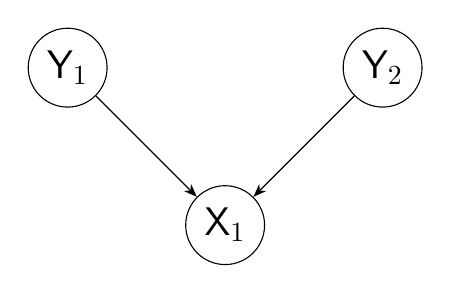
\begin{tikzpicture}[
        >=Stealth,
        node distance=2.8cm,
        every node/.style={
            circle,
            draw,
            minimum size=1cm,
            font=\Large
        }
    ]
    
    \node (Y1) at (0,2) {$\mathsf{Y}_1$};
    \node (Y2) at (4,2) {$\mathsf{Y}_2$};
    \node (X1) at (2,0) {$\mathsf{X}_1$};
    
    \draw[->] (Y1) -- (X1);
    \draw[->] (Y2) -- (X1);

    \end{tikzpicture}
    \caption{Bayesian network with two parent registers and one child
    register.}
    \label{fig:bn}
    \end{figure}

We denote the associated spaces by
$\mathcal{X}_{1}=\mathbb{C}^{\Sigma_{1}}$ and
$\mathcal{Y}_{i}=\mathbb{C}^{\Gamma_{i}}$ for $i\in\{1,2\}$. To avoid
repeating the two parent registers in every expression, let
\begin{equation}
    \mathbf{Y}=(\mathsf{Y}_{1},\mathsf{Y}_{2}),
    \qquad
    \boldsymbol{\Gamma}=\Gamma_{1}\times\Gamma_{2},
    \qquad
    \mathcal{Y}=\mathcal{Y}_{1}\otimes\mathcal{Y}_{2}.
\end{equation}
For $\mathbf{y}=(y_{1},y_{2})\in\boldsymbol{\Gamma}$, we also write
\begin{equation}
    E_{\mathbf{y}}
    =
    E_{y_{1},y_{1}}\otimes E_{y_{2},y_{2}}.
\end{equation}
The conditional distribution can then be viewed as the pointwise function
\begin{equation}
    p_{\mathsf{X}_{1}|\mathbf{Y}}:
    \Sigma_{1}\times\boldsymbol{\Gamma}
    \to[0,1],
\end{equation}
where
$p_{\mathsf{X}_{1}|\mathbf{Y}}(x|\mathbf{y})
=p_{\mathsf{X}_{1}|\mathsf{Y}_{1},\mathsf{Y}_{2}}
(x|y_{1},y_{2})$.

The corresponding Choi state is
\begin{equation}
    \rho_{\mathsf{X}_{1}|\mathbf{Y}}
    =
    \sum_{x\in\Sigma_{1}}
    \sum_{\mathbf{y}\in\boldsymbol{\Gamma}}
    p_{\mathsf{X}_{1}|\mathbf{Y}}(x|\mathbf{y})
    \bigl(E_{x,x}\otimes E_{\mathbf{y}}\bigr),
\end{equation}
where
$\rho_{\mathsf{X}_{1}|\mathbf{Y}}
\equiv
\rho_{\mathsf{X}_{1}|\mathsf{Y}_{1},\mathsf{Y}_{2}}$.
Its normalization is
\begin{equation}
    \mathrm{Tr}_{\mathcal{X}_{1}}
    \bigl(\rho_{\mathsf{X}_{1}|\mathbf{Y}}\bigr)
    =
    \mathrm{Id}_{\mathcal{Y}}.
\end{equation}
It therefore defines the quantum stochastic map
\begin{equation}
    \Phi_{\mathsf{X}_{1}|\mathbf{Y}}:
    L(\mathcal{Y})
    \to
    L(\mathcal{X}_{1})
\end{equation}
given by
\begin{equation}
    \Phi_{\mathsf{X}_{1}|\mathbf{Y}}(A)
    =
    \mathrm{Tr}_{\mathcal{Y}}
    \left(
        \rho_{\mathsf{X}_{1}|\mathbf{Y}}
        \bigl(
            \mathrm{Id}_{\mathcal{X}_{1}}\otimes A^{T}
        \bigr)
    \right).
\end{equation}

Since $\mathsf{Y}_{1}$ and $\mathsf{Y}_{2}$ are independent root
registers, their joint state factorizes as
\begin{equation}
    \rho_{\mathbf{Y}}
    =
    \rho_{\mathsf{Y}_{1}}\otimes\rho_{\mathsf{Y}_{2}}
    =
    \bigotimes_{i=1}^{2}
    \left(
        \sum_{y_{i}\in\Gamma_{i}}
        p_{\mathsf{Y}_{i}}(y_{i})E_{y_{i},y_{i}}
    \right).
\end{equation}

Applying the map to the joint state of the parent registers gives the
state of the child register:
\begin{equation}
    \Phi_{\mathsf{X}_{1}|\mathbf{Y}}
    \left(\rho_{\mathbf{Y}}\right)
    =
    \rho_{\mathsf{X}_{1}}.
\end{equation}

\subsubsection{Two child registers with one parent}
\label{subsubsec:BN2}
We now consider the registers
$\mathsf{X}_{1},\mathsf{X}_{2},\mathsf{Y}$ with the Bayesian network shown
in Fig.~\ref{fig:bn2}.

\begin{figure}[ht]
    \centering
    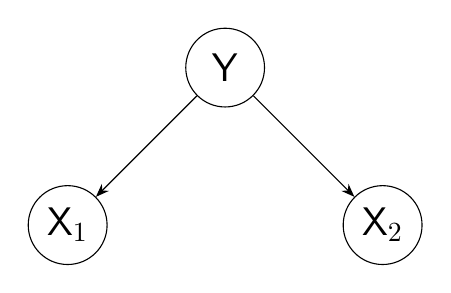
\begin{tikzpicture}[
        >=Stealth,
        node distance=2.8cm,
        every node/.style={
            circle,
            draw,
            minimum size=1cm,
            font=\Large
        }
    ]
    
    \node (Y1) at (4,2) {$\mathsf{Y}$};
    \node (X1) at (2,0) {$\mathsf{X}_1$};
    \node (X2) at (6,0) {$\mathsf{X}_2$};
    
    \draw[->] (Y1) -- (X1);
    
    \draw[->] (Y1) -- (X2);

    
    \end{tikzpicture}
    \caption{Bayesian network with one parent register and two child
    registers.}
    \label{fig:bn2}
    \end{figure}

We denote the associated spaces by
$\mathcal{X}_{i}=\mathbb{C}^{\Sigma_{i}}$ for $i\in\{1,2\}$ and
$\mathcal{Y}=\mathbb{C}^{\Gamma}$. As in the preceding example, it is useful
to group the two child registers:
\begin{equation}
    \mathbf{X}=(\mathsf{X}_{1},\mathsf{X}_{2}),
    \qquad
    \boldsymbol{\Sigma}=\Sigma_{1}\times\Sigma_{2},
    \qquad
    \mathcal{X}=\mathcal{X}_{1}\otimes\mathcal{X}_{2}.
\end{equation}
For $\mathbf{x}=(x_{1},x_{2})\in\boldsymbol{\Sigma}$, define
\begin{equation}
    E_{\mathbf{x}}
    =
    E_{x_{1},x_{1}}\otimes E_{x_{2},x_{2}}.
\end{equation}
The conditional operator is then
\begin{equation}
    \rho_{\mathbf{X}|\mathsf{Y}}
    =
    \sum_{\mathbf{x}\in\boldsymbol{\Sigma}}
    \sum_{y\in\Gamma}
    p_{\mathbf{X}|\mathsf{Y}}(\mathbf{x}|y)
    \bigl(E_{\mathbf{x}}\otimes E_{y,y}\bigr),
\end{equation}
where
$\rho_{\mathbf{X}|\mathsf{Y}}
\equiv\rho_{\mathsf{X}_{1},\mathsf{X}_{2}|\mathsf{Y}}$ and
$p_{\mathbf{X}|\mathsf{Y}}(\mathbf{x}|y)
=p_{\mathsf{X}_{1},\mathsf{X}_{2}|\mathsf{Y}}(x_{1},x_{2}|y)$.
We are also interested in the two conditional Choi states
$\rho_{\mathsf{X}_{1}|\mathsf{Y}}$ and
$\rho_{\mathsf{X}_{2}|\mathsf{Y}}$. They are obtained by reducing
$\rho_{\mathbf{X}|\mathsf{Y}}$. For example, the partial trace over
$\mathcal{X}_{2}$ is
\begin{equation}
    \mathrm{Tr}_{\mathcal{X}_{2}}
    =
    \mathrm{Id}_{L(\mathcal{X}_{1})}
    \otimes\mathrm{Tr}
    \otimes\mathrm{Id}_{L(\mathcal{Y})}.
\end{equation}
Applying it gives
\begin{equation}
    \mathrm{Tr}_{\mathcal{X}_{2}}
    \bigl(\rho_{\mathbf{X}|\mathsf{Y}}\bigr)=
    \sum_{\mathbf{x}\in\boldsymbol{\Sigma}}
    \sum_{y\in\Gamma}
    p_{\mathbf{X}|\mathsf{Y}}(\mathbf{x}|y)
    \bigl(E_{x_{1},x_{1}}\otimes E_{y,y}\bigr).
\end{equation}
Using the classical conditional marginalization
\begin{equation}
    p_{\mathsf{X}_{1}|\mathsf{Y}}(x_{1}|y)
    =
    \sum_{x_{2}\in\Sigma_{2}}
    p_{\mathbf{X}|\mathsf{Y}}\bigl((x_{1},x_{2})|y\bigr),
\end{equation}
we obtain
\begin{align}
    \mathrm{Tr}_{\mathcal{X}_{2}}
    \bigl(\rho_{\mathbf{X}|\mathsf{Y}}\bigr)
    &=
    \sum_{x_{1}\in\Sigma_{1}}\sum_{y\in\Gamma}
    p_{\mathsf{X}_{1}|\mathsf{Y}}(x_{1}|y)
    \bigl(E_{x_{1},x_{1}}\otimes E_{y,y}\bigr)\\
    &=
    \rho_{\mathsf{X}_{1}|\mathsf{Y}}.
\end{align}
Using the same argument, we have
\begin{equation}
    \mathrm{Tr}_{\mathcal{X}_{1}}
    \bigl(\rho_{\mathbf{X}|\mathsf{Y}}\bigr)
    =
    \rho_{\mathsf{X}_{2}|\mathsf{Y}}.
\end{equation}
These reductions are the operator analogue of conditional marginalization.

The three Choi states live in different operator spaces:
\begin{align}
    \rho_{\mathsf{X}_{1}|\mathsf{Y}}
    &\in L(\mathcal{X}_{1}\otimes\mathcal{Y}),\\
    \rho_{\mathsf{X}_{2}|\mathsf{Y}}
    &\in L(\mathcal{X}_{2}\otimes\mathcal{Y}),\\
    \rho_{\mathbf{X}|\mathsf{Y}}
    &\in L(\mathcal{X}\otimes\mathcal{Y}).
\end{align}
Their corresponding stochastic maps satisfy
\begin{equation}
    \begin{aligned}
    \Phi_{\mathsf{X}_{i}|\mathsf{Y}}
    &\in T(\mathcal{Y},\mathcal{X}_{i}),
    &&i\in\{1,2\},\\
    \Phi_{\mathbf{X}|\mathsf{Y}}
    &\in T(\mathcal{Y},\mathcal{X}),
    \end{aligned}
\end{equation}
and
\begin{align}
    \Phi_{\mathsf{X}_{i}|\mathsf{Y}}(\rho_{\mathsf{Y}})
    &=
    \rho_{\mathsf{X}_{i}},
    &&i\in\{1,2\},\\
    \Phi_{\mathbf{X}|\mathsf{Y}}(\rho_{\mathsf{Y}})
    &=
    \rho_{\mathbf{X}}.
\end{align}

Since $\Phi_{\mathbf{X}|\mathsf{Y}}$ gives the joint state of the two child
registers, we can compose it with a partial trace to obtain either marginal
state. For example,
\begin{equation}
    \mathrm{Tr}_{\mathcal{X}_{1}}
    \circ\Phi_{\mathbf{X}|\mathsf{Y}}:
    L(\mathcal{Y})
    \to
    L(\mathcal{X}_{2}),
\end{equation}
and therefore
\begin{equation}
    \bigl(
        \mathrm{Tr}_{\mathcal{X}_{1}}
        \circ\Phi_{\mathbf{X}|\mathsf{Y}}
    \bigr)(\rho_{\mathsf{Y}})
    =
    \rho_{\mathsf{X}_{2}}.
\end{equation}
We call this composition a \emph{marginal quantum stochastic map} and
denote it by
\begin{equation}
    \Phi_{\mathbf{X}|\mathsf{Y}}^{\mathcal{X}_{1}}
    :=
    \mathrm{Tr}_{\mathcal{X}_{1}}
    \circ\Phi_{\mathbf{X}|\mathsf{Y}}.
\end{equation}
Its full form is
\begin{equation}
    \Phi_{\mathbf{X}|\mathsf{Y}}^{\mathcal{X}_{1}}(A)
    =
    \mathrm{Tr}_{\mathcal{X}_{1}}
    \Bigl(
        \mathrm{Tr}_{\mathcal{Y}}
        \bigl(
            \rho_{\mathbf{X}|\mathsf{Y}}(\mathrm{Id}_{\mathcal{X}}\otimes A^{T})
        \bigr)
    \Bigr).
\end{equation}
The same construction applies when $\mathcal{X}_{2}$ is traced out.

A natural question is whether the two conditional operators can be
combined to recover $\rho_{\mathbf{X}|\mathsf{Y}}$. In this classical
setting the answer is yes. The graph implies the conditional independence
$\mathsf{X}_{1}\perp\mathsf{X}_{2}\mid\mathsf{Y}$, and therefore
\begin{equation}
    p_{\mathbf{X}|\mathsf{Y}}(\mathbf{x}|y)
    =
    p_{\mathsf{X}_{1}|\mathsf{Y}}(x_{1}|y)
    p_{\mathsf{X}_{2}|\mathsf{Y}}(x_{2}|y).
\end{equation}
We first lift each conditional operator to
$L(\mathcal{X}\otimes\mathcal{Y})$ by defining
\begin{equation}
    \sigma_{\mathsf{X}_{1}|\mathsf{Y}}
    =
    \sum_{x_{1}\in\Sigma_{1}}\sum_{y\in\Gamma}
    p_{\mathsf{X}_{1}|\mathsf{Y}}(x_{1}|y)
    \bigl(
        E_{x_{1},x_{1}}
        \otimes\mathrm{Id}_{\mathcal{X}_{2}}
        \otimes E_{y,y}
    \bigr),
\end{equation}
and
\begin{equation}
    \sigma_{\mathsf{X}_{2}|\mathsf{Y}}
    =
    \sum_{x_{2}\in\Sigma_{2}}\sum_{y'\in\Gamma}
    p_{\mathsf{X}_{2}|\mathsf{Y}}(x_{2}|y')
    \bigl(
        \mathrm{Id}_{\mathcal{X}_{1}}
        \otimes E_{x_{2},x_{2}}
        \otimes E_{y',y'}
    \bigr).
\end{equation}
These operators are diagonal, so they commute. Their matrix product gives
\begin{align}
    \sigma_{\mathsf{X}_{1}|\mathsf{Y}}
    \sigma_{\mathsf{X}_{2}|\mathsf{Y}}
    &=
    \sum_{\mathbf{x}\in\boldsymbol{\Sigma}}
    \sum_{y,y'\in\Gamma}
    p_{\mathsf{X}_{1}|\mathsf{Y}}(x_{1}|y)
    p_{\mathsf{X}_{2}|\mathsf{Y}}(x_{2}|y')
    \notag\\[-0.25em]
    &\qquad\cdot
    \bigl(
        E_{\mathbf{x}}\otimes E_{y,y}E_{y',y'}
    \bigr)\\
    &=
    \sum_{\mathbf{x}\in\boldsymbol{\Sigma}}
    \sum_{y,y'\in\Gamma}
    p_{\mathsf{X}_{1}|\mathsf{Y}}(x_{1}|y)
    p_{\mathsf{X}_{2}|\mathsf{Y}}(x_{2}|y')
    \notag\\[-0.25em]
    &\qquad\cdot
    \bigl(
        E_{\mathbf{x}}\otimes
        \delta_{y,y'}E_{y',y'}
    \bigr)\\
    &=
    \sum_{\mathbf{x}\in\boldsymbol{\Sigma}}
    \sum_{y\in\Gamma}
    p_{\mathsf{X}_{1}|\mathsf{Y}}(x_{1}|y)
    p_{\mathsf{X}_{2}|\mathsf{Y}}(x_{2}|y)
    \notag\\[-0.25em]
    &\qquad\cdot
    \bigl(E_{\mathbf{x}}\otimes E_{y,y}\bigr)
    \label{eq:factor-equation}\\
    &=
    \sum_{\mathbf{x}\in\boldsymbol{\Sigma}}
    \sum_{y\in\Gamma}
    p_{\mathbf{X}|\mathsf{Y}}(\mathbf{x}|y)
    \bigl(E_{\mathbf{x}}\otimes E_{y,y}\bigr)\\
    &=
    \rho_{\mathbf{X}|\mathsf{Y}}.
\end{align}
Hence, after placing the two operators in the common space
$L(\mathcal{X}\otimes\mathcal{Y})$, their matrix product recovers the joint
conditional Choi state:
\begin{equation}
    \sigma_{\mathsf{X}_{1}|\mathsf{Y}}
    \sigma_{\mathsf{X}_{2}|\mathsf{Y}}
    =
    \rho_{\mathbf{X}|\mathsf{Y}}.
\end{equation}

\paragraph{Factor products.}

The preceding calculation is the operator representation of the product of
two factors~\cite[Sec.~11.3.1]{Darwiche2008}. Let
$A:\Sigma_{1}\times\Gamma\to\mathbb{R}$ and
$B:\Sigma_{2}\times\Gamma\to\mathbb{R}$ be factors with
\begin{equation}
    \mathrm{Var}(A)=
    \bigl\{\mathsf{X}_{1},\mathsf{Y}\bigr\},
    \qquad
    \mathrm{Var}(B)=
    \bigl\{\mathsf{X}_{2},\mathsf{Y}\bigr\}.
\end{equation}
Set
$\boldsymbol{\Omega}=\Sigma_{1}\times\Sigma_{2}\times\Gamma$.
Their product is the factor
\begin{equation}
    C:
    \boldsymbol{\Omega}
    \to\mathbb{R}.
\end{equation}
For every joint assignment
$\mathbf{z}=(x_{1},x_{2},y)\in\boldsymbol{\Omega}$, let $\mathbf{z}'$ and
$\mathbf{z}''$ denote its restrictions to $\mathrm{Var}(A)$ and
$\mathrm{Var}(B)$, respectively.
The product factor is then defined by
\begin{equation}
    C(\mathbf{z})
    =
    A(\mathbf{z}')B(\mathbf{z}'').
\end{equation}
If
\begin{equation}
    E_{\mathbf{z}}
    =
    E_{\mathbf{x}}\otimes E_{y,y},
\end{equation}
the diagonal operator associated with $C$ is
\begin{equation}
    \begin{aligned}
    R_{C}
    &=
    \sum_{\mathbf{z}\in\boldsymbol{\Omega}}
    A(\mathbf{z}')B(\mathbf{z}'')E_{\mathbf{z}}\\
    &=
    \sum_{\mathbf{z}\in\boldsymbol{\Omega}}
    C(\mathbf{z})E_{\mathbf{z}}.
    \end{aligned}
\end{equation}
For the two-child network in Fig.~\ref{fig:bn2}, we take
$A=p_{\mathsf{X}_{1}|\mathsf{Y}}$ and
$B=p_{\mathsf{X}_{2}|\mathsf{Y}}$. Conditional independence gives
$C=p_{\mathbf{X}|\mathsf{Y}}$, so that
$R_{C}=\rho_{\mathbf{X}|\mathsf{Y}}$, as shown explicitly in
Eq.~\eqref{eq:factor-equation}.

\subsubsection{Conditional Choi operators for compound registers}

We can now introduce the notation for an arbitrary collection of child and
parent registers. Let
$\mathsf{X}_{1},\dots,\mathsf{X}_{m}$ be the child registers and
$\mathsf{Y}_{1},\dots,\mathsf{Y}_{n}$ the parent registers. We write
\begin{equation}
    \mathbf{X}=(\mathsf{X}_{1},\dots,\mathsf{X}_{m}),
    \qquad
    \mathbf{Y}=(\mathsf{Y}_{1},\dots,\mathsf{Y}_{n}).
\end{equation}
For each register, let
$\mathcal{X}_{i}=\mathbb{C}^{\Sigma_{i}}$ for
$i\in\{1,\dots,m\}$ and
$\mathcal{Y}_{j}=\mathbb{C}^{\Gamma_{j}}$ for
$j\in\{1,\dots,n\}$. The compound alphabets and spaces are
\begin{align}
    \boldsymbol{\Sigma}
    &=
    \Sigma_{1}\times\cdots\times\Sigma_{m},
    &
    \mathcal{X}
    &=
    \bigotimes_{i=1}^{m}\mathcal{X}_{i},\\
    \boldsymbol{\Gamma}
    &=
    \Gamma_{1}\times\cdots\times\Gamma_{n},
    &
    \mathcal{Y}
    &=
    \bigotimes_{j=1}^{n}\mathcal{Y}_{j}.
\end{align}
For realizations of these registers, we use
\begin{equation}
    \mathbf{x}=(x_{1},\dots,x_{m})
    \in\boldsymbol{\Sigma},
    \qquad
    \mathbf{y}=(y_{1},\dots,y_{n})
    \in\boldsymbol{\Gamma},
\end{equation}
and define
\begin{equation}
    E_{\mathbf{x}}
    =
    \bigotimes_{i=1}^{m}E_{x_{i},x_{i}},
    \qquad
    E_{\mathbf{y}}
    =
    \bigotimes_{j=1}^{n}E_{y_{j},y_{j}}.
\end{equation}
The conditional distribution
\begin{equation}
    p_{\mathbf{X}|\mathbf{Y}}:
    \boldsymbol{\Sigma}\times\boldsymbol{\Gamma}
    \to[0,1]
\end{equation}
is therefore represented by the conditional Choi state
\begin{equation}
    \rho_{\mathbf{X}|\mathbf{Y}}
    =
    \sum_{\mathbf{x}\in\boldsymbol{\Sigma}}
    \sum_{\mathbf{y}\in\boldsymbol{\Gamma}}
    p_{\mathbf{X}|\mathbf{Y}}(\mathbf{x}|\mathbf{y})
    \bigl(E_{\mathbf{x}}\otimes E_{\mathbf{y}}\bigr).
\end{equation}
It belongs to $L(\mathcal{X}\otimes\mathcal{Y})$ and satisfies
\begin{equation}
    \mathrm{Tr}_{\mathcal{X}}
    \bigl(\rho_{\mathbf{X}|\mathbf{Y}}\bigr)
    =
    \mathrm{Id}_{\mathcal{Y}}.
\end{equation}


\subsection{Quantum Channel Networks and Q-Factors}
\label{subsection:qbn1}

We now consider networks composed only of quantum registers and quantum
channels. These networks form the purely quantum fragment of the Q-factor
framework introduced by Di Guardia, Ehrhard, and
Faggian~\cite[Defs.~13 and~19]{DiGuardiaEhrhardFaggian2026}. In the absence
of classical variables, a Q-factor is a positive operator. When its partial
trace over the output space is the identity on the input space, it is the
Choi operator of a quantum channel. The networks studied here are therefore
quantum channel networks rather than full quantum Bayesian networks.

\subsubsection{Quantum registers and channel Q-factors}

We use the register conventions introduced in
Section~\ref{sec:quantum-state}. For a quantum register $\mathsf{Q}$, its
associated complex Euclidean space will be denoted by
$\mathcal{H}_{\mathsf{Q}}$. In particular, if
$\mathsf{Q}=(q_{1},\dots,q_{n})$ is an $n$-qubit register, then
\begin{equation}
    \mathcal{H}_{\mathsf{Q}}
    =
    \bigotimes_{r=1}^{n}\mathcal{H}_{q_{r}}
    \cong
    \mathbb{C}^{2^{n}}.
\end{equation}
We also use bra-ket notation whenever a basis representation is required.
If $\{\ket{a}\}$ is the chosen basis, then $\ket{a}\bra{b}$ denotes the
corresponding matrix unit; in particular, for
$\mathcal{X}=\mathbb{C}^{\Sigma}$, we identify $\ket{a}=e_a$ and
$\ket{a}\bra{b}=E_{a,b}$.

\subsubsection{A single-channel network}

Consider the following channel network:
\begin{figure}[ht]
    \centering
    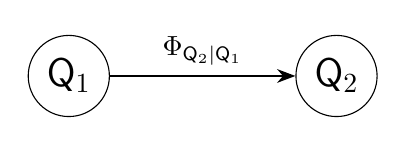
\begin{tikzpicture}[
        >=Stealth,
        node/.style={
            circle,
            draw,
            minimum size=1cm,
            font=\Large
        }
    ]
        \node[node] (Q1) at (0,0) {$\mathsf{Q}_{1}$};
        \node[node] (Q2) at (3.4,0) {$\mathsf{Q}_{2}$};
        \draw[->, thick] (Q1) --
            node[midway,above] {$\Phi_{\mathsf{Q}_{2}|\mathsf{Q}_{1}}$}
            (Q2);
    \end{tikzpicture}
    \caption{A single-channel network from $\mathsf{Q}_{1}$ to
    $\mathsf{Q}_{2}$.}
    \label{fig:qbn}
\end{figure}

We associate a Q-factor with each register:
\begin{enumerate}
    \item The initial factor is the state
    $\rho_{\mathsf{Q}_{1}}\in D(\mathcal{H}_{\mathsf{Q}_{1}})$.

    \item The factor associated with $\mathsf{Q}_{2}$ is
    \begin{equation}
        \rho_{\mathsf{Q}_{2}|\mathsf{Q}_{1}}
        \in
        \mathrm{Pos}\left(
            \mathcal{H}_{\mathsf{Q}_{2}}
            \otimes
            \mathcal{H}_{\mathsf{Q}_{1}}
        \right),
    \end{equation}
    with
    \begin{equation}
        \mathrm{Tr}_{\mathcal{H}_{\mathsf{Q}_{2}}}
        \left(
            \rho_{\mathsf{Q}_{2}|\mathsf{Q}_{1}}
        \right)
        =
        \mathrm{Id}_{\mathcal{H}_{\mathsf{Q}_{1}}}.
    \end{equation}
\end{enumerate}
The second factor is positive and satisfies the partial-trace normalization
above. It is therefore the Choi operator of the unique quantum channel
\begin{equation}
    \Phi_{\mathsf{Q}_{2}|\mathsf{Q}_{1}}:
    L(\mathcal{H}_{\mathsf{Q}_{1}})
    \to
    L(\mathcal{H}_{\mathsf{Q}_{2}}).
\end{equation}
When the input is $\rho_{\mathsf{Q}_{1}}$, the resulting state is
\begin{equation}
    \Phi_{\mathsf{Q}_{2}|\mathsf{Q}_{1}}
    \left(\rho_{\mathsf{Q}_{1}}\right)
    =
    \rho_{\mathsf{Q}_{2}}.
\end{equation}
Using the Choi action formula established earlier, the channel is given
by~\cite[Eqs.~(2.65)--(2.66)]{Watrous2018}
\begin{equation}
    \Phi_{\mathsf{Q}_{2}|\mathsf{Q}_{1}}(\cdot)
    =
    \mathrm{Tr}_{\mathcal{H}_{\mathsf{Q}_{1}}}
    \left(
        \rho_{\mathsf{Q}_{2}|\mathsf{Q}_{1}}
        \left(
            \mathrm{Id}_{\mathcal{H}_{\mathsf{Q}_{2}}}
            \otimes
            (\cdot)^{T}
        \right)
    \right).
\end{equation}
Thus, one first transposes the input operator in the chosen basis. The
operator
\begin{equation}
    \mathrm{Id}_{\mathcal{H}_{\mathsf{Q}_{2}}}
    \otimes
    \rho_{\mathsf{Q}_{1}}^{T}
    \label{eq:lifted-operator-1}
\end{equation}
lifts $\rho_{\mathsf{Q}_{1}}^{T}$ to
$L(\mathcal{H}_{\mathsf{Q}_{2}}\otimes
\mathcal{H}_{\mathsf{Q}_{1}})$. It can then be multiplied by the Choi
operator:
\begin{equation}
    \rho_{\mathsf{Q}_{2}|\mathsf{Q}_{1}}
    \left(
        \mathrm{Id}_{\mathcal{H}_{\mathsf{Q}_{2}}}
        \otimes
        \rho_{\mathsf{Q}_{1}}^{T}
    \right)
    \in
    L\left(
        \mathcal{H}_{\mathsf{Q}_{2}}
        \otimes
        \mathcal{H}_{\mathsf{Q}_{1}}
    \right).
\end{equation}
Finally, tracing out $\mathcal{H}_{\mathsf{Q}_{1}}$ gives the output
density operator $\rho_{\mathsf{Q}_{2}}$.

\subsubsection{Block-matrix form of the Choi action}

Let $\mathcal{H}_{1}=\mathbb{C}^{2}$ and fix the computational basis
$\{\ket{0},\ket{1}\}$. A normalized pure state
$\ket{\psi}\in\mathcal{H}_{1}$ determines the density operator
$\rho=\ket{\psi}\bra{\psi}$.

\begin{example}
    \label{ex:choi-computation}
    Write
    \begin{equation}
        \ket{\psi}
        =
        \sum_{r=0}^{1}c_{r}\ket{r}
        =
        c_{0}\ket{0}+c_{1}\ket{1},
    \end{equation}
    where $|c_{0}|^{2}+|c_{1}|^{2}=1$. The corresponding density
    operator is
    \begin{equation}
        \begin{aligned}
        \rho
        &=
        (c_{0}\ket{0}+c_{1}\ket{1})
        (c_{0}^{*}\bra{0}+c_{1}^{*}\bra{1})\\
        &=
        \begin{pmatrix}
            |c_{0}|^{2} & c_{0}c_{1}^{*} \\
            c_{1}c_{0}^{*} & |c_{1}|^{2}
        \end{pmatrix}.
        \end{aligned}
    \end{equation}
    For the remainder of the example, we regard $\rho$ as the
    transpose of an input state $\gamma\in D(\mathcal{H}_{1})$, so
    that $\rho=\gamma^{T}$. Let
    $\mathcal{H}_{2}\cong\mathbb{C}^{2}$ be another qubit space and
    define
    $\hat{\rho}\in
    L(\mathcal{H}_{2}\otimes\mathcal{H}_{1})$ by
    \begin{align}
        \hat{\rho}
        &=
        \mathrm{Id}_{\mathcal{H}_{2}}\otimes\rho\notag\\
        &=
        \begin{pmatrix}
            1&0\\
            0&1
        \end{pmatrix}
        \otimes
        \begin{pmatrix}
            |c_{0}|^{2} & c_{0}c_{1}^{*}\\
            c_{1}c_{0}^{*} & |c_{1}|^{2}
        \end{pmatrix}\notag\\
        &=
        \left(
        \begin{array}{c|c}
            \rho&\mathbf{0}\\ \hline
            \mathbf{0}&\rho
        \end{array}
        \right)\notag\\
        &=
        \left(
        \begin{array}{cc|cc}
            |c_{0}|^{2}&c_{0}c_{1}^{*}&0&0\\
            c_{1}c_{0}^{*}&|c_{1}|^{2}&0&0\\ \hline
            0&0&|c_{0}|^{2}&c_{0}c_{1}^{*}\\
            0&0&c_{1}c_{0}^{*}&|c_{1}|^{2}
        \end{array}
        \right).
        \label{eq:lifting-operation}
    \end{align}
    This is precisely the lifted operator in
    Eq.~\eqref{eq:lifted-operator-1}.

    Now let $\sigma\in
    L(\mathcal{H}_{2}\otimes\mathcal{H}_{1})$ be the Choi operator
    \begin{equation}
        \sigma
        =
        \left(
        \begin{array}{cc|cc}
            a&b&c&d\\
            e&f&g&h\\ \hline
            i&j&k&l\\
            m&n&o&p
        \end{array}
        \right).
        \label{eq:choi-state-1}
    \end{equation}
    The entries are symbolic, but they are constrained by
    \begin{equation}
        \sigma\in
        \mathrm{Pos}(\mathcal{H}_{2}\otimes\mathcal{H}_{1}),
        \qquad
        \mathrm{Tr}_{\mathcal{H}_{2}}(\sigma)
        =
        \mathrm{Id}_{\mathcal{H}_{1}}.
    \end{equation}
    In the channel network above, $\sigma$ plays the role of
    $\rho_{\mathsf{Q}_{2}|\mathsf{Q}_{1}}$. Decompose it into blocks:
    \begin{equation}
        \sigma
        =
        \left(
        \begin{array}{c|c}
            A&B\\ \hline
            C&D
        \end{array}
        \right),
    \end{equation}
    where
    \begin{equation}
        \begin{gathered}
        A=
        \begin{pmatrix}
            a&b\\
            e&f
        \end{pmatrix},
        \qquad
        B=
        \begin{pmatrix}
            c&d\\
            g&h
        \end{pmatrix},\\
        C=
        \begin{pmatrix}
            i&j\\
            m&n
        \end{pmatrix},
        \qquad
        D=
        \begin{pmatrix}
            k&l\\
            o&p
        \end{pmatrix}.
        \end{gathered}
    \end{equation}
    Matrix multiplication gives
    \begin{equation}
        \sigma\hat{\rho}
        =
        \begin{pmatrix}
            A&B\\
            C&D
        \end{pmatrix}
        \begin{pmatrix}
            \rho&0\\
            0&\rho
        \end{pmatrix}
        =
        \begin{pmatrix}
            A\rho&B\rho\\
            C\rho&D\rho
        \end{pmatrix}.
    \end{equation}
    The partial trace over $\mathcal{H}_{1}$ is therefore
    \begin{equation}
        \mathrm{Tr}_{\mathcal{H}_{1}}(\sigma\hat{\rho})
        =
        \begin{pmatrix}
            \mathrm{Tr}(A\rho)&\mathrm{Tr}(B\rho)\\
            \mathrm{Tr}(C\rho)&\mathrm{Tr}(D\rho)
        \end{pmatrix}.
        \label{eq:pt}
    \end{equation}
    For example,
    \begin{equation}
        \begin{aligned}
        A\rho
        &=
        \begin{pmatrix}
            a&b\\
            e&f
        \end{pmatrix}
        \begin{pmatrix}
            |c_{0}|^{2}&c_{0}c_{1}^{*}\\
            c_{1}c_{0}^{*}&|c_{1}|^{2}
        \end{pmatrix}\\
        &=
        \begin{pmatrix}
            a|c_{0}|^{2}+bc_{1}c_{0}^{*}&\star\\
            \star&ec_{0}c_{1}^{*}+f|c_{1}|^{2}
        \end{pmatrix},
        \end{aligned}
    \end{equation}
    where the entries denoted by $\star$ do not contribute to the
    trace.

    Consequently,
    \begin{align}
        \mathrm{Tr}(A\rho)
        &=
        a|c_{0}|^{2}
        +bc_{1}c_{0}^{*}
        +ec_{0}c_{1}^{*}
        +f|c_{1}|^{2}.
        \\
        \mathrm{Tr}_{\mathcal{H}_{1}}(\sigma\hat{\rho})
        &=
        \begin{pmatrix}
        \begin{gathered}
        a|c_0|^2+b\,c_1c_0^*\\
        {}+e\,c_0c_1^*+f|c_1|^2
        \end{gathered}
        &
        \begin{gathered}
        c|c_0|^2+d\,c_1c_0^*\\
        {}+g\,c_0c_1^*+h|c_1|^2
        \end{gathered}
        \\[2.5ex]
        \begin{gathered}
        i|c_0|^2+j\,c_1c_0^*\\
        {}+m\,c_0c_1^*+n|c_1|^2
        \end{gathered}
        &
        \begin{gathered}
        k|c_0|^2+l\,c_1c_0^*\\
        {}+o\,c_0c_1^*+p|c_1|^2
        \end{gathered}
        \end{pmatrix}.
        \label{eq:pt2}
    \end{align}
    Here, the matrix entry $i$ is an arbitrary complex number and
    should not be confused with the imaginary unit.
\end{example}

\subsubsection{Choi action as a tensor contraction}
\label{subsubsec:Mat-Gt}

A natural question is whether we really need to perform all the
preceding operations in order to obtain the output of the map
$\Phi_{\mathsf{Q}_{2}|\mathsf{Q}_{1}}$. We first transpose the input
matrix, lift it to the space of the Choi operator so that the matrix
multiplication can be performed, and finally apply the partial trace. Is
there a more direct way to carry out this computation?

The operator--tensor correspondence introduced in the preliminaries
allows us to express the same calculation as a tensor contraction.
Accordingly, the operators $\sigma$ and $\hat{\rho}$ are represented by
tensors $\sigma'$ and $\hat{\rho}'$, respectively. Relative to the
factorization into the two subsystems, these are tensors of type $(2,2)$
(order four):
\begin{equation}
    \sigma',\hat{\rho}'
    \in
    (\mathcal{H}_{2}\otimes\mathcal{H}_{1})
    \otimes
    (\mathcal{H}_{2}\otimes\mathcal{H}_{1})^{*}.
\end{equation}

Throughout this subsection, we use the standard tensor-calculus
convention introduced in the preliminaries: a repeated index is
contracted only when it occurs once in an upper position and once in a
lower position. To distinguish tensors from the operators they
represent, square brackets will be reserved for the component matrix of
a tensor. To obtain the matrix representations of $\sigma'$ and
$\hat{\rho}'$, we use the canonical basis
\begin{equation}
    \mathcal{B}
    =
    \left\{
        \ket{i_{2}i_{1}}\bra{j_{2}j_{1}}
        :
        i_{2},i_{1},j_{2},j_{1}\in\{0,1\}
    \right\}.
\end{equation}
The pairs $(i_{2},j_{2})$ and $(i_{1},j_{1})$ correspond to
$\mathcal{H}_{2}$ and $\mathcal{H}_{1}$, respectively. We set
\begin{equation*}
    [\sigma']_{\mathcal{B}}=\sigma,
    \qquad
    [\hat{\rho}']_{\mathcal{B}}=\hat{\rho},
\end{equation*}
where the operators on the right are written in this canonical basis.
Thus,
\begin{equation}
    \sigma'
    =
    \sum_{i_{2},i_{1},j_{2},j_{1}}
    (\sigma')^{i_{2}i_{1}}{}_{j_{2}j_{1}}
    \ket{i_{2}i_{1}}\bra{j_{2}j_{1}},
\end{equation}
and its matrix representation is
\begin{equation}
    [\sigma']_{\mathcal{B}}
    =
    \begin{pmatrix}
        (\sigma')^{00}{}_{00}&(\sigma')^{00}{}_{01}&
        (\sigma')^{00}{}_{10}&(\sigma')^{00}{}_{11}\\
        (\sigma')^{01}{}_{00}&(\sigma')^{01}{}_{01}&
        (\sigma')^{01}{}_{10}&(\sigma')^{01}{}_{11}\\
        (\sigma')^{10}{}_{00}&(\sigma')^{10}{}_{01}&
        (\sigma')^{10}{}_{10}&(\sigma')^{10}{}_{11}\\
        (\sigma')^{11}{}_{00}&(\sigma')^{11}{}_{01}&
        (\sigma')^{11}{}_{10}&(\sigma')^{11}{}_{11}
    \end{pmatrix}.
\end{equation}
Ordinary matrix multiplication is represented by the upper--lower
contraction
\begin{equation}
    \varphi^{i_{2}i_{1}}{}_{m_{2}m_{1}}
    =
    (\sigma')^{i_{2}i_{1}}{}_{j_{2}j_{1}}
    (\hat{\rho}')^{j_{2}j_{1}}{}_{m_{2}m_{1}},
\end{equation}
or, with the sums displayed,
\begin{equation}
    \varphi^{i_{2}i_{1}}{}_{m_{2}m_{1}}
    =
    \sum_{j_{2},j_{1}}
    (\sigma')^{i_{2}i_{1}}{}_{j_{2}j_{1}}
    (\hat{\rho}')^{j_{2}j_{1}}{}_{m_{2}m_{1}}.
\end{equation}

The tensor $\varphi$ therefore satisfies
$[\varphi]_{\mathcal{B}}=\sigma\hat{\rho}$. Its full component matrix
is
\begin{equation}
    [\varphi]_{\mathcal{B}}=\begin{pmatrix}
        \varphi^{\color{brown}0\color{green!60!black}0}{}_{\color{brown}0\color{green!60!black}0} & \varphi^{\color{brown}0\color{green!60!black}0}{}_{\color{brown}0\color{green!60!black}1} & \varphi^{\color{brown}0\color{green!60!black}0}{}_{\color{brown}1\color{green!60!black}0} & \varphi^{\color{brown}0\color{green!60!black}0}{}_{\color{brown}1\color{green!60!black}1} \\ 
        \varphi^{\color{brown}0\color{green!60!black}1}{}_{\color{brown}0\color{green!60!black}0} & \varphi^{\color{brown}0\color{green!60!black}1}{}_{\color{brown}0\color{green!60!black}1} & \varphi^{\color{brown}0\color{green!60!black}1}{}_{\color{brown}1\color{green!60!black}0} & \varphi^{\color{brown}0\color{green!60!black}1}{}_{\color{brown}1\color{green!60!black}1} \\ 
        \varphi^{\color{brown}1\color{green!60!black}0}{}_{\color{brown}0\color{green!60!black}0} & \varphi^{\color{brown}1\color{green!60!black}0}{}_{\color{brown}0\color{green!60!black}1} & \varphi^{\color{brown}1\color{green!60!black}0}{}_{\color{brown}1\color{green!60!black}0} & \varphi^{\color{brown}1\color{green!60!black}0}{}_{\color{brown}1\color{green!60!black}1}\\
        \varphi^{\color{brown}1\color{green!60!black}1}{}_{\color{brown}0\color{green!60!black}0} & \varphi^{\color{brown}1\color{green!60!black}1}{}_{\color{brown}0\color{green!60!black}1} & \varphi^{\color{brown}1\color{green!60!black}1}{}_{\color{brown}1\color{green!60!black}0} & \varphi^{\color{brown}1\color{green!60!black}1}{}_{\color{brown}1\color{green!60!black}1}  
\end{pmatrix}
\end{equation}
The brown indices refer to $\mathcal{H}_{2}$, while the green indices
refer to $\mathcal{H}_{1}$. It is useful to view this order-four tensor
as a $2\times2$ array of $2\times2$ blocks. For fixed
$i_{2},j_{2}\in\{0,1\}$, define
\begin{equation}
    \varphi^{i_{2}}{}_{j_{2}}
    \coloneqq
    \begin{pmatrix}
        \varphi^{i_{2}0}{}_{j_{2}0}&
        \varphi^{i_{2}0}{}_{j_{2}1}\\
        \varphi^{i_{2}1}{}_{j_{2}0}&
        \varphi^{i_{2}1}{}_{j_{2}1}
    \end{pmatrix}.
\end{equation}
\begin{figure}[ht]
    \centering

\[ \begin{pmatrix}
    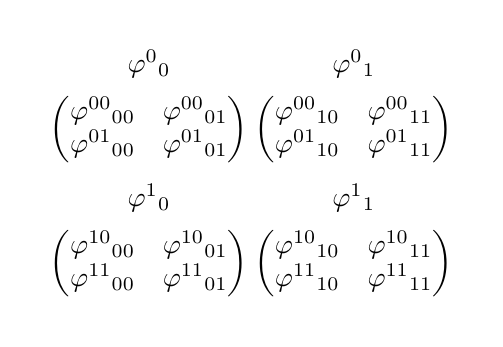
\begin{tikzpicture}[
        block/.style={
            align=center,
            inner sep=8pt
        }
    ]
    
    \node[block] (A) at (0,1.8) {
        $\varphi^{0}{}_{0}$\\[2mm]
        $\begin{pmatrix}
            \varphi^{00}{}_{00} & \varphi^{00}{}_{01}\\
            \varphi^{01}{}_{00} & \varphi^{01}{}_{01}
        \end{pmatrix}$
    };
    
    \node[block] (B) at (2.6,1.8) {
        $\varphi^{0}{}_{1}$\\[2mm]
        $\begin{pmatrix}
            \varphi^{00}{}_{10} & \varphi^{00}{}_{11}\\
            \varphi^{01}{}_{10} & \varphi^{01}{}_{11}
        \end{pmatrix}$
    };
    
    \node[block] (C) at (0,0.1) {
        $\varphi^{1}{}_{0}$\\[2mm]
        $\begin{pmatrix}
            \varphi^{10}{}_{00} & \varphi^{10}{}_{01}\\
            \varphi^{11}{}_{00} & \varphi^{11}{}_{01}
        \end{pmatrix}$
    };
    
    \node[block] (D) at (2.6,0.1) {
        $\varphi^{1}{}_{1}$\\[2mm]
        $\begin{pmatrix}
            \varphi^{10}{}_{10} & \varphi^{10}{}_{11}\\
            \varphi^{11}{}_{10} & \varphi^{11}{}_{11}
        \end{pmatrix}$
    };


    \end{tikzpicture}
\end{pmatrix}
\]
    
\caption{The tensor $\varphi$ represented as a $2\times2$ array
of $2\times2$ matrices.}    \label{fig:rank-four-tensor}

\end{figure} 

The reason the representation in Fig.~\ref{fig:rank-four-tensor} is
useful is that the partial trace over $\mathcal{H}_{1}$ is obtained by
taking the ordinary trace of each block
$\varphi^{i_{2}}{}_{j_{2}}$. Indeed, for the operator represented by
$[\varphi]_{\mathcal{B}}$,
\begin{equation}
    \left(
        \mathrm{Tr}_{\mathcal{H}_{1}}(\varphi)
    \right)^{i_{2}}{}_{j_{2}}
    =
    \mathrm{Tr}\left(\varphi^{i_{2}}{}_{j_{2}}\right)
    =
    \varphi^{i_{2}i_{1}}{}_{j_{2}i_{1}}.
\end{equation}
The result is a tensor of type $(1,1)$ on $\mathcal{H}_{2}$ and agrees
with Eq.~\eqref{eq:pt2}. Indeed,
$[\sigma']_{\mathcal{B}}$ and $[\hat{\rho}']_{\mathcal{B}}$ are the
operator matrices in Eqs.~\eqref{eq:choi-state-1} and
\eqref{eq:lifting-operation}. Relative to the canonical basis
\begin{equation}
    \mathcal{A}
    =
    \left\{
        \ket{i_{2}}\bra{j_{2}}
        :
        i_{2},j_{2}\in\{0,1\}
    \right\}
\end{equation}
of $L(\mathcal{H}_{2})$, one has
\begin{equation}
    \left[
        \mathrm{Tr}_{\mathcal{H}_{1}}(\varphi)
    \right]_{\mathcal{A}}
    =
    \mathrm{Tr}_{\mathcal{H}_{1}}
    \left(
        [\sigma']_{\mathcal{B}}
        [\hat{\rho}']_{\mathcal{B}}
    \right).
\end{equation}

We can now bypass the lifted matrix. Let
\begin{equation}
    \mathcal{A}'
    =
    \left\{
        \ket{i_{1}}\bra{j_{1}}
        :
        i_{1},j_{1}\in\{0,1\}
    \right\}
\end{equation}
be the canonical basis of $L(\mathcal{H}_{1})$, and write the
components of $\rho$ as $\rho^{i_{1}}{}_{j_{1}}$. Direct contraction
with the input indices of $\sigma'$ defines
\begin{equation}
    \chi^{i_{2}}{}_{j_{2}}
    =
    (\sigma')^{i_{2}i_{1}}{}_{j_{2}j_{1}}
    \rho^{j_{1}}{}_{i_{1}}.
\end{equation}
The exchanged indices of $\rho$ account for the transpose in the Choi
action. More explicitly,
\begin{align}
    (\sigma')^{i_{2}i_{1}}{}_{j_{2}j_{1}}
    \rho^{j_{1}}{}_{i_{1}}
    &=
    \sum_{i_{1}}\sum_{j_{1}}
    (\sigma')^{i_{2}i_{1}}{}_{j_{2}j_{1}}
    \rho^{j_{1}}{}_{i_{1}}\\
    &=
    \sum_{i_{1}}
    \left(
        (\sigma')^{i_{2}i_{1}}{}_{j_{2}0}
        \rho^{0}{}_{i_{1}}
        +
        (\sigma')^{i_{2}i_{1}}{}_{j_{2}1}
        \rho^{1}{}_{i_{1}}
    \right)\\
    &=
    (\sigma')^{i_{2}0}{}_{j_{2}0}\rho^{0}{}_{0}
    +
    (\sigma')^{i_{2}0}{}_{j_{2}1}\rho^{1}{}_{0}
    \nonumber\\
    &\quad+
    (\sigma')^{i_{2}1}{}_{j_{2}0}\rho^{0}{}_{1}
    +
    (\sigma')^{i_{2}1}{}_{j_{2}1}\rho^{1}{}_{1}.
\end{align}
For example, the first two entries of the output are
\begin{align}
    \chi^{0}{}_{0}
    &=
    (\sigma')^{00}{}_{00}\rho^{0}{}_{0}
    +
    (\sigma')^{00}{}_{01}\rho^{1}{}_{0}
    \nonumber\\
    &\quad+
    (\sigma')^{01}{}_{00}\rho^{0}{}_{1}
    +
    (\sigma')^{01}{}_{01}\rho^{1}{}_{1}\\
    &=
    a|c_{0}|^{2}
    +bc_{1}c_{0}^{*}
    +ec_{0}c_{1}^{*}
    +f|c_{1}|^{2},\\
    \chi^{0}{}_{1}
    &=
    (\sigma')^{00}{}_{10}\rho^{0}{}_{0}
    +
    (\sigma')^{00}{}_{11}\rho^{1}{}_{0}
    \nonumber\\
    &\quad+
    (\sigma')^{01}{}_{10}\rho^{0}{}_{1}
    +
    (\sigma')^{01}{}_{11}\rho^{1}{}_{1}\\
    &=
    c|c_{0}|^{2}
    +dc_{1}c_{0}^{*}
    +gc_{0}c_{1}^{*}
    +h|c_{1}|^{2}.
\end{align}
These are precisely the corresponding entries of Eq.~\eqref{eq:pt2}.
Therefore,
\begin{equation}
    \begin{aligned}
    \chi^{i_{2}}{}_{j_{2}}
    &=
    \left(
        \mathrm{Tr}_{\mathcal{H}_{1}}
        (\sigma\hat{\rho})
    \right)^{i_{2}}{}_{j_{2}}\\
    &=
    \left(
        \mathrm{Tr}_{\mathcal{H}_{1}}
        \left(
            \sigma
            (\mathrm{Id}_{\mathcal{H}_{2}}\otimes\rho)
        \right)
    \right)^{i_{2}}{}_{j_{2}}.
    \end{aligned}
\end{equation}

\begin{proposition}[Choi action as a tensor contraction]
    \label{prop:choi-action-tensor-contraction}
    Let
    \begin{equation}
        \Phi_{\mathsf{Q}_{2}|\mathsf{Q}_{1}}:
        L(\mathcal{H}_{\mathsf{Q}_{1}})
        \to
        L(\mathcal{H}_{\mathsf{Q}_{2}})
    \end{equation}
    be a quantum channel with Choi operator
    $\rho_{\mathsf{Q}_{2}|\mathsf{Q}_{1}}$. Let
    \begin{equation}
        \rho'_{\mathsf{Q}_{2}|\mathsf{Q}_{1}}
        \in
        (\mathcal{H}_{\mathsf{Q}_{2}}
        \otimes\mathcal{H}_{\mathsf{Q}_{1}})
        \otimes
        (\mathcal{H}_{\mathsf{Q}_{2}}
        \otimes\mathcal{H}_{\mathsf{Q}_{1}})^{*}
    \end{equation}
    be the tensor representing this Choi operator. For
    $\rho_{\mathsf{Q}_{1}}\in
    D(\mathcal{H}_{\mathsf{Q}_{1}})$, let
    $\rho'_{\mathsf{Q}_{1}}\in
    \mathcal{H}_{\mathsf{Q}_{1}}
    \otimes\mathcal{H}_{\mathsf{Q}_{1}}^{*}$ represent the transposed
    input state. If $\mathcal{C}$, $\mathcal{B}$, and $\mathcal{B}'$
    are the canonical bases of the corresponding operator spaces, then
    \begin{equation}
        \left[
            \rho'_{\mathsf{Q}_{2}|\mathsf{Q}_{1}}
        \right]_{\mathcal{C}}
        =
        \rho_{\mathsf{Q}_{2}|\mathsf{Q}_{1}},
        \qquad
        \left[
            \rho'_{\mathsf{Q}_{1}}
        \right]_{\mathcal{B}}
        =
        \rho_{\mathsf{Q}_{1}}^{T}.
    \end{equation}
    The tensor $\rho'_{\mathsf{Q}_{2}}\in
    \mathcal{H}_{\mathsf{Q}_{2}}
    \otimes\mathcal{H}_{\mathsf{Q}_{2}}^{*}$ defined by
    \begin{equation}
        (\rho'_{\mathsf{Q}_{2}})^{i_{2}}{}_{j_{2}}
        =
        (\rho'_{\mathsf{Q}_{2}|\mathsf{Q}_{1}})
        ^{i_{2}i_{1}}{}_{j_{2}j_{1}}
        (\rho'_{\mathsf{Q}_{1}})^{j_{1}}{}_{i_{1}}
    \end{equation}
    represents the output state. In other words,
    \begin{equation}
        \left[
            \rho'_{\mathsf{Q}_{2}}
        \right]_{\mathcal{B}'}
        =
        \Phi_{\mathsf{Q}_{2}|\mathsf{Q}_{1}}
        \left(\rho_{\mathsf{Q}_{1}}\right)
        =
        \rho_{\mathsf{Q}_{2}}.
    \end{equation}
\end{proposition}

\begin{proof}[Proof sketch]
        The inverse Choi--Jamio{\l}kowski formula gives
        \begin{equation}
            \left(
                \Phi_{\mathsf{Q}_{2}|\mathsf{Q}_{1}}
                \left(\rho_{\mathsf{Q}_{1}}\right)
            \right)^{i_{2}}{}_{j_{2}}
            =
            (\rho'_{\mathsf{Q}_{2}|\mathsf{Q}_{1}})
            ^{i_{2}i_{1}}{}_{j_{2}j_{1}}
            (\rho'_{\mathsf{Q}_{1}})^{j_{1}}{}_{i_{1}}.
        \end{equation}
        This proves the stated contraction identity. For the qubit
        channel considered in Example~\ref{ex:choi-computation}, the
        same identity can be verified explicitly as follows. Let
        \begin{equation}
            \hat{\rho}_{\mathsf{Q}_{1}}
            \in
            (\mathcal{H}_{\mathsf{Q}_{2}}
            \otimes\mathcal{H}_{\mathsf{Q}_{1}})
            \otimes
            (\mathcal{H}_{\mathsf{Q}_{2}}
            \otimes\mathcal{H}_{\mathsf{Q}_{1}})^{*}
        \end{equation}
        be the lifted tensor satisfying
        \begin{equation}
            [\hat{\rho}_{\mathsf{Q}_{1}}]_{\mathcal{C}}
            =
            \mathrm{Id}_{\mathcal{H}_{\mathsf{Q}_{2}}}
            \otimes
            \rho_{\mathsf{Q}_{1}}^{T}.
        \end{equation}
        Its complete component matrix is
        \begin{equation}
        [\hat{\rho}_{\mathsf{Q}_{1}}]_{\mathcal{C}}
        =
        \begin{pmatrix}
        (\hat{\rho}_{\mathsf{Q}_{1}})^{\color{brown}0\color{blue}0}{}_{\color{brown}0\color{blue}0}&
        (\hat{\rho}_{\mathsf{Q}_{1}})^{\color{brown}0\color{blue}0}{}_{\color{brown}0\color{blue}1}&
        (\hat{\rho}_{\mathsf{Q}_{1}})^{\color{brown}0\color{blue}0}{}_{\color{brown}1\color{blue}0}&
        (\hat{\rho}_{\mathsf{Q}_{1}})^{\color{brown}0\color{blue}0}{}_{\color{brown}1\color{blue}1}\\
        (\hat{\rho}_{\mathsf{Q}_{1}})^{\color{brown}0\color{blue}1}{}_{\color{brown}0\color{blue}0}&
        (\hat{\rho}_{\mathsf{Q}_{1}})^{\color{brown}0\color{blue}1}{}_{\color{brown}0\color{blue}1}&
        (\hat{\rho}_{\mathsf{Q}_{1}})^{\color{brown}0\color{blue}1}{}_{\color{brown}1\color{blue}0}&
        (\hat{\rho}_{\mathsf{Q}_{1}})^{\color{brown}0\color{blue}1}{}_{\color{brown}1\color{blue}1}\\
        (\hat{\rho}_{\mathsf{Q}_{1}})^{\color{brown}1\color{blue}0}{}_{\color{brown}0\color{blue}0}&
        (\hat{\rho}_{\mathsf{Q}_{1}})^{\color{brown}1\color{blue}0}{}_{\color{brown}0\color{blue}1}&
        (\hat{\rho}_{\mathsf{Q}_{1}})^{\color{brown}1\color{blue}0}{}_{\color{brown}1\color{blue}0}&
        (\hat{\rho}_{\mathsf{Q}_{1}})^{\color{brown}1\color{blue}0}{}_{\color{brown}1\color{blue}1}\\
        (\hat{\rho}_{\mathsf{Q}_{1}})^{\color{brown}1\color{blue}1}{}_{\color{brown}0\color{blue}0}&
        (\hat{\rho}_{\mathsf{Q}_{1}})^{\color{brown}1\color{blue}1}{}_{\color{brown}0\color{blue}1}&
        (\hat{\rho}_{\mathsf{Q}_{1}})^{\color{brown}1\color{blue}1}{}_{\color{brown}1\color{blue}0}&
        (\hat{\rho}_{\mathsf{Q}_{1}})^{\color{brown}1\color{blue}1}{}_{\color{brown}1\color{blue}1}
        \end{pmatrix}.
        \end{equation}
        Its two off-diagonal blocks satisfy
        \begin{equation}
        \begin{aligned}
        \begin{pmatrix}
        (\hat{\rho}_{\mathsf{Q}_{1}})^{\color{brown}0\color{blue}0}{}_{\color{brown}1\color{blue}0}&
        (\hat{\rho}_{\mathsf{Q}_{1}})^{\color{brown}0\color{blue}0}{}_{\color{brown}1\color{blue}1}\\
        (\hat{\rho}_{\mathsf{Q}_{1}})^{\color{brown}0\color{blue}1}{}_{\color{brown}1\color{blue}0}&
        (\hat{\rho}_{\mathsf{Q}_{1}})^{\color{brown}0\color{blue}1}{}_{\color{brown}1\color{blue}1}
        \end{pmatrix}
        &=
        \begin{pmatrix}
        (\hat{\rho}_{\mathsf{Q}_{1}})^{\color{brown}1\color{blue}0}{}_{\color{brown}0\color{blue}0}&
        (\hat{\rho}_{\mathsf{Q}_{1}})^{\color{brown}1\color{blue}0}{}_{\color{brown}0\color{blue}1}\\
        (\hat{\rho}_{\mathsf{Q}_{1}})^{\color{brown}1\color{blue}1}{}_{\color{brown}0\color{blue}0}&
        (\hat{\rho}_{\mathsf{Q}_{1}})^{\color{brown}1\color{blue}1}{}_{\color{brown}0\color{blue}1}
        \end{pmatrix}\\
        &=
        \begin{pmatrix}
            0&0\\
            0&0
        \end{pmatrix}.
        \end{aligned}
        \end{equation}
        Thus $[\hat{\rho}_{\mathsf{Q}_{1}}]_{\mathcal{C}}$ is
        block diagonal. Componentwise,
        \begin{equation}
            (\hat{\rho}_{\mathsf{Q}_{1}})
            ^{\color{brown}i_{2}\color{blue}i_{1}}
            {}_{\color{brown}j_{2}\color{blue}j_{1}}
            =
            \begin{cases}
                0,
                &\color{brown}i_{2}\neq j_{2},\\
                (\rho'_{\mathsf{Q}_{1}})
                ^{\color{blue}i_{1}}{}_{\color{blue}j_{1}},
                &\color{brown}i_{2}=j_{2}.
            \end{cases}
        \end{equation}
        Equivalently,
        \begin{equation}
            (\hat{\rho}_{\mathsf{Q}_{1}})
            ^{\color{brown}i_{2}\color{blue}i_{1}}
            {}_{\color{brown}j_{2}\color{blue}j_{1}}
            =
            \delta^{\color{brown}i_{2}}{}_{\color{brown}j_{2}}
            (\rho'_{\mathsf{Q}_{1}})
            ^{\color{blue}i_{1}}{}_{\color{blue}j_{1}}.
            \label{eq:kronecker-expre}
        \end{equation}
        This is exactly the tensor form of
        $\mathrm{Id}_{\mathcal{H}_{\mathsf{Q}_{2}}}
        \otimes\rho_{\mathsf{Q}_{1}}^{T}$.

        The contraction
        \begin{equation}
            (\rho'_{\mathsf{Q}_{2}|\mathsf{Q}_{1}})
            ^{i_{2}i_{1}}{}_{j_{2}j_{1}}
            (\hat{\rho}_{\mathsf{Q}_{1}})
            ^{j_{2}j_{1}}{}_{m_{2}m_{1}}
        \end{equation}
        is the component form of the matrix product
        \begin{equation}
            \left(
                \rho_{\mathsf{Q}_{2}|\mathsf{Q}_{1}}
                \left(
                    \mathrm{Id}_{\mathcal{H}_{\mathsf{Q}_{2}}}
                    \otimes
                    \rho_{\mathsf{Q}_{1}}^{T}
                \right)
            \right)_{ij}=
            (\rho_{\mathsf{Q}_{2}|\mathsf{Q}_{1}})_{ik}
            \left(
                \mathrm{Id}_{\mathcal{H}_{\mathsf{Q}_{2}}}
                \otimes
                \rho_{\mathsf{Q}_{1}}^{T}
            \right)_{kj}.
        \end{equation}
        Applying the partial trace over $\mathsf{Q}_{1}$ identifies
        $m_{1}$ with $i_{1}$:
        \begin{equation}
            (\rho'_{\mathsf{Q}_{2}|\mathsf{Q}_{1}})
            ^{i_{2}i_{1}}{}_{j_{2}j_{1}}
            (\hat{\rho}_{\mathsf{Q}_{1}})
            ^{j_{2}j_{1}}{}_{m_{2}i_{1}}.
        \end{equation}
        Hence
        \begin{equation}
            (\rho'_{\mathsf{Q}_{2}})^{i_{2}}{}_{m_{2}}
            =
            (\rho'_{\mathsf{Q}_{2}|\mathsf{Q}_{1}})
            ^{i_{2}i_{1}}{}_{j_{2}j_{1}}
            (\hat{\rho}_{\mathsf{Q}_{1}})
            ^{j_{2}j_{1}}{}_{m_{2}i_{1}}.
        \end{equation}
        Substituting expression~\eqref{eq:kronecker-expre} gives
        \begin{equation}
        \begin{aligned}
        &(\rho'_{\mathsf{Q}_{2}|\mathsf{Q}_{1}})
        ^{i_{2}i_{1}}{}_{j_{2}j_{1}}
        (\hat{\rho}_{\mathsf{Q}_{1}})
        ^{j_{2}j_{1}}{}_{m_{2}m_{1}}\\
        &\quad=
        (\rho'_{\mathsf{Q}_{2}|\mathsf{Q}_{1}})
        ^{i_{2}i_{1}}{}_{j_{2}j_{1}}
        \delta^{j_{2}}{}_{m_{2}}
        (\rho'_{\mathsf{Q}_{1}})^{j_{1}}{}_{m_{1}}\\
        &\quad=
        (\rho'_{\mathsf{Q}_{2}|\mathsf{Q}_{1}})
        ^{i_{2}i_{1}}{}_{m_{2}j_{1}}
        (\rho'_{\mathsf{Q}_{1}})^{j_{1}}{}_{m_{1}}.
        \end{aligned}
        \end{equation}
        Define
        \begin{equation}
            \varphi^{i_{2}i_{1}}{}_{m_{2}m_{1}}
            =
            (\rho'_{\mathsf{Q}_{2}|\mathsf{Q}_{1}})
            ^{i_{2}i_{1}}{}_{m_{2}j_{1}}
            (\rho'_{\mathsf{Q}_{1}})^{j_{1}}{}_{m_{1}}.
        \end{equation}
        Taking the partial trace gives
        \begin{equation}
            \left(
                \mathrm{Tr}_{\mathcal{H}_{\mathsf{Q}_{1}}}
                (\varphi)
            \right)^{i_{2}}{}_{m_{2}}
            =
            (\rho'_{\mathsf{Q}_{2}|\mathsf{Q}_{1}})
            ^{i_{2}i_{1}}{}_{m_{2}j_{1}}
            (\rho'_{\mathsf{Q}_{1}})^{j_{1}}{}_{i_{1}}.
        \end{equation}
        Therefore,
        \begin{equation}
            \begin{aligned}
            (\rho'_{\mathsf{Q}_{2}})^{i_{2}}{}_{m_{2}}
            &=
            (\rho'_{\mathsf{Q}_{2}|\mathsf{Q}_{1}})
            ^{i_{2}i_{1}}{}_{j_{2}j_{1}}
            (\hat{\rho}_{\mathsf{Q}_{1}})
            ^{j_{2}j_{1}}{}_{m_{2}i_{1}}\\
            &=
            (\rho'_{\mathsf{Q}_{2}|\mathsf{Q}_{1}})
            ^{i_{2}i_{1}}{}_{m_{2}j_{1}}
            (\rho'_{\mathsf{Q}_{1}})^{j_{1}}{}_{i_{1}}.
            \end{aligned}
        \end{equation}
\end{proof}

The Choi action is therefore obtained directly by contracting the indices of
the input register. This single contraction encodes both the multiplication
by the lifted transposed input and the subsequent partial trace.

\subsubsection{Composition of channel Q-factors}
\label{subsubsec:pqf}

Channel composition can also be expressed directly in terms of Choi
operators through the link product~\cite{ChiribellaDArianoPerinotti2009}.
Here we work with tensor components in order to keep the contraction over
the intermediate register explicit.

Consider the chain of two quantum channels shown in
Fig.~\ref{fig:qbn1}.
\par
\begin{figure}[ht]
    \centering
    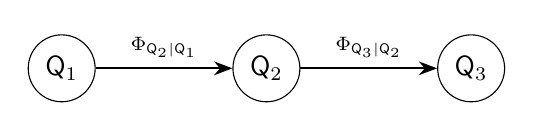
\begin{tikzpicture}[
        >=Stealth,
        node/.style={
            circle,
            draw,
            minimum size=0.85cm,
            font=\normalsize
        }
    ]
        \node[node] (Q1) at (0,0) {$\mathsf{Q}_{1}$};
        \node[node] (Q2) at (2.6,0) {$\mathsf{Q}_{2}$};
        \node[node] (Q3) at (5.2,0) {$\mathsf{Q}_{3}$};
        \draw[->, thick] (Q1) --
            node[midway,above,font=\scriptsize]
            {$\Phi_{\mathsf{Q}_{2}|\mathsf{Q}_{1}}$}
            (Q2);
        \draw[->, thick] (Q2) --
            node[midway,above,font=\scriptsize]
            {$\Phi_{\mathsf{Q}_{3}|\mathsf{Q}_{2}}$}
            (Q3);
    \end{tikzpicture}
    \caption{A two-channel chain.}
    \label{fig:qbn1}
\end{figure}
\par
The associated Q-factors are
\begin{enumerate}
    \item
    $\rho_{\mathsf{Q}_{1}}
    \in D(\mathcal{H}_{\mathsf{Q}_{1}})$;

    \item
    $\rho_{\mathsf{Q}_{2}|\mathsf{Q}_{1}}
    \in
    \mathrm{Pos}(
        \mathcal{H}_{\mathsf{Q}_{2}}
        \otimes
        \mathcal{H}_{\mathsf{Q}_{1}}
    )$, with
    \begin{equation}
        \mathrm{Tr}_{\mathcal{H}_{\mathsf{Q}_{2}}}
        \left(
            \rho_{\mathsf{Q}_{2}|\mathsf{Q}_{1}}
        \right)
        =
        \mathrm{Id}_{\mathcal{H}_{\mathsf{Q}_{1}}};
    \end{equation}

    \item
    $\rho_{\mathsf{Q}_{3}|\mathsf{Q}_{2}}
    \in
    \mathrm{Pos}(
        \mathcal{H}_{\mathsf{Q}_{3}}
        \otimes
        \mathcal{H}_{\mathsf{Q}_{2}}
    )$, with
    \begin{equation}
        \mathrm{Tr}_{\mathcal{H}_{\mathsf{Q}_{3}}}
        \left(
            \rho_{\mathsf{Q}_{3}|\mathsf{Q}_{2}}
        \right)
        =
        \mathrm{Id}_{\mathcal{H}_{\mathsf{Q}_{2}}}.
    \end{equation}
\end{enumerate}
The last two factors are the Choi operators of the corresponding
channels. Their component contraction is the pure-quantum instance of
the product of Q-factors~\cite[Def.~17]{DiGuardiaEhrhardFaggian2026}.

For this example, $\mathsf{Q}_{1}$, $\mathsf{Q}_{2}$, and
$\mathsf{Q}_{3}$ are qubit registers. Each index $i_{r},j_{r}$ is associated
with $\mathcal{H}_{\mathsf{Q}_{r}}$ and takes values in $\{0,1\}$. The
corresponding tensors are
\begin{enumerate}
    \item
    $\varrho_{\mathsf{Q}_{1}}
    \in
    \mathcal{H}_{\mathsf{Q}_{1}}
    \otimes
    \mathcal{H}_{\mathsf{Q}_{1}}^{*}$, with components
    $(\varrho_{\mathsf{Q}_{1}})^{i_{1}}{}_{j_{1}}$;

    \item
    $\varrho_{\mathsf{Q}_{2}|\mathsf{Q}_{1}}
    \in
    (\mathcal{H}_{\mathsf{Q}_{2}}
    \otimes\mathcal{H}_{\mathsf{Q}_{1}})
    \otimes
    (\mathcal{H}_{\mathsf{Q}_{2}}
    \otimes\mathcal{H}_{\mathsf{Q}_{1}})^{*}$, with components
    $(\varrho_{\mathsf{Q}_{2}|\mathsf{Q}_{1}})
    ^{i_{2}i_{1}}{}_{j_{2}j_{1}}$;

    \item
    $\varrho_{\mathsf{Q}_{3}|\mathsf{Q}_{2}}
    \in
    (\mathcal{H}_{\mathsf{Q}_{3}}
    \otimes\mathcal{H}_{\mathsf{Q}_{2}})
    \otimes
    (\mathcal{H}_{\mathsf{Q}_{3}}
    \otimes\mathcal{H}_{\mathsf{Q}_{2}})^{*}$, with components
    $(\varrho_{\mathsf{Q}_{3}|\mathsf{Q}_{2}})
    ^{i_{3}i_{2}}{}_{j_{3}j_{2}}$.
\end{enumerate}
Let $\mathcal{B}^{(r)}$ denote the canonical basis of
$L(\mathcal{H}_{\mathsf{Q}_{r}})$, let $\mathcal{A}$ denote the
canonical basis of
$L(\mathcal{H}_{\mathsf{Q}_{2}}\otimes
\mathcal{H}_{\mathsf{Q}_{1}})$, and let $\mathcal{A}'$ denote the
canonical basis of
$L(\mathcal{H}_{\mathsf{Q}_{3}}\otimes
\mathcal{H}_{\mathsf{Q}_{2}})$. We set
\begin{equation}
    \begin{gathered}
    [\varrho_{\mathsf{Q}_{1}}]_{\mathcal{B}^{(1)}}
    =
    \rho_{\mathsf{Q}_{1}}^{T},\\
    [\varrho_{\mathsf{Q}_{2}|\mathsf{Q}_{1}}]_{\mathcal{A}}
    =
    \rho_{\mathsf{Q}_{2}|\mathsf{Q}_{1}},
    \qquad
    [\varrho_{\mathsf{Q}_{3}|\mathsf{Q}_{2}}]_{\mathcal{A}'}
    =
    \rho_{\mathsf{Q}_{3}|\mathsf{Q}_{2}}.
    \end{gathered}
\end{equation}
and
\begin{equation}
    [\varrho_{\mathsf{Q}_{2}}]_{\mathcal{B}^{(2)}}
    =
    \rho_{\mathsf{Q}_{2}},
    \qquad
    [\varrho_{\mathsf{Q}_{3}}]_{\mathcal{B}^{(3)}}
    =
    \rho_{\mathsf{Q}_{3}}.
    \label{eq:teq1}
\end{equation}

Before writing the component contraction, consider the two channels
\begin{equation}
    \Phi_{\mathsf{Q}_{2}|\mathsf{Q}_{1}},
    \qquad
    \Phi_{\mathsf{Q}_{3}|\mathsf{Q}_{2}}.
\end{equation}
Their composition satisfies
\begin{equation}
    \left(
        \Phi_{\mathsf{Q}_{3}|\mathsf{Q}_{2}}
        \circ
        \Phi_{\mathsf{Q}_{2}|\mathsf{Q}_{1}}
    \right)
    \left(\rho_{\mathsf{Q}_{1}}\right)
    =
    \rho_{\mathsf{Q}_{3}}.
\end{equation}
Applying the Choi action formula successively gives
\begin{equation}
\begin{aligned}
\rho_{\mathsf{Q}_{2}}
&=
\mathrm{Tr}_{\mathcal{H}_{\mathsf{Q}_{1}}}
\left(
    \rho_{\mathsf{Q}_{2}|\mathsf{Q}_{1}}
    \left(
        \mathrm{Id}_{\mathcal{H}_{\mathsf{Q}_{2}}}
        \otimes
        \rho_{\mathsf{Q}_{1}}^{T}
    \right)
\right),\\
\left(
    \Phi_{\mathsf{Q}_{3}|\mathsf{Q}_{2}}
    \circ
    \Phi_{\mathsf{Q}_{2}|\mathsf{Q}_{1}}
\right)
\left(\rho_{\mathsf{Q}_{1}}\right)
&=
\mathrm{Tr}_{\mathcal{H}_{\mathsf{Q}_{2}}}
\left(
    \rho_{\mathsf{Q}_{3}|\mathsf{Q}_{2}}
    \left(
        \mathrm{Id}_{\mathcal{H}_{\mathsf{Q}_{3}}}
        \otimes
        \rho_{\mathsf{Q}_{2}}^{T}
    \right)
\right).
\end{aligned}
\label{eq:composition-choi-maps}
\end{equation}

Can we express this composition with tensors? As we saw in
Section~\ref{subsubsec:Mat-Gt},
\begin{equation}
    \left(\varrho_{\mathsf{Q}_{2}}\right)^{i_{2}}{}_{j_{2}}
    =
    \left(\varrho_{\mathsf{Q}_{1}}\right)^{j_{1}}{}_{i_{1}}
    \left(\varrho_{\mathsf{Q}_{2}|\mathsf{Q}_{1}}\right)
    ^{i_{2}i_{1}}{}_{j_{2}j_{1}}.
    \label{eq:teq2}
\end{equation}
But can we find $\varrho_{\mathsf{Q}_{3}}$ while keeping our definition
of $\varrho_{\mathsf{Q}_{2}}$? The composition of the maps in
Eq.~\eqref{eq:composition-choi-maps} would formally take the form
\begin{equation}
    \left(\varrho_{\mathsf{Q}_{3}}\right)^{i_{3}}{}_{j_{3}}=
    \left(\varrho_{\mathsf{Q}_{2}|\mathsf{Q}_{1}}\right)
    ^{i_{2}i_{1}}{}_{j_{2}j_{1}}
    \left(\varrho_{\mathsf{Q}_{3}|\mathsf{Q}_{2}}\right)
    ^{i_{3}i_{2}}{}_{j_{3}j_{2}}
    \left(\varrho_{\mathsf{Q}_{1}}\right)^{j_{1}}{}_{i_{1}}.
\end{equation}
Using Eq.~\eqref{eq:teq2}, this would reduce to
\begin{equation}
    \left(\varrho_{\mathsf{Q}_{3}}\right)^{i_{3}}{}_{j_{3}}
    =
    \left(\varrho_{\mathsf{Q}_{2}}\right)^{i_{2}}{}_{j_{2}}
    \left(\varrho_{\mathsf{Q}_{3}|\mathsf{Q}_{2}}\right)
    ^{i_{3}i_{2}}{}_{j_{3}j_{2}}.
    \label{eq:teq3}
\end{equation}
At this point, however, we encounter a problem. In
Eq.~\eqref{eq:teq3}, $i_{2}$ occurs twice in the upper position and
$j_{2}$ twice in the lower position. Therefore, this is not a tensor
contraction according to the standard upper--lower convention used so
far. Moreover, if the repeated indices are summed directly, the
expression is not covariant under arbitrary changes of basis. This
difficulty comes from the transpose of the intermediate state in the
Choi action.

To retain our definition of $\varrho_{\mathsf{Q}_{2}}$ and compose the
channel factors directly, we now fix an orthonormal basis for each register,
taking the computational basis for qubit registers
\cite[Secs.~6.1--6.3]{DullemondPeeters2010}. We retain the mixed
placement of upper and lower indices to indicate row and column indices,
but from this point onward a repeated register index is summed over even
when both occurrences are upper indices or both are lower indices.
With this convention, the two preceding expressions are valid component
identities in these bases. In
particular, the contraction in Eq.~\eqref{eq:teq3} absorbs the transpose
of the intermediate state.

To see explicitly how the transpose is encoded, define
$\varsigma_{\mathsf{Q}_{1}}\in
\mathcal{H}_{\mathsf{Q}_{1}}\otimes
\mathcal{H}_{\mathsf{Q}_{1}}^{*}$ by
\begin{equation}
    [\varsigma_{\mathsf{Q}_{1}}]_{\mathcal{B}^{(1)}}
    =
    \rho_{\mathsf{Q}_{1}}.
\end{equation}
Then
\begin{equation}
    \left(\varrho_{\mathsf{Q}_{1}}\right)^{j_{1}}{}_{i_{1}}
    =
    \left(\varsigma_{\mathsf{Q}_{1}}\right)^{i_{1}}{}_{j_{1}},
\end{equation}
and Eq.~\eqref{eq:teq2} becomes
\begin{equation}
    \left(\varrho_{\mathsf{Q}_{2}}\right)^{i_{2}}{}_{j_{2}}
    =
    \left(\varsigma_{\mathsf{Q}_{1}}\right)^{i_{1}}{}_{j_{1}}
    \left(\varrho_{\mathsf{Q}_{2}|\mathsf{Q}_{1}}\right)
    ^{i_{2}i_{1}}{}_{j_{2}j_{1}}.
    \label{eq:teq4}
\end{equation}
This has exactly the same contraction pattern as
Eq.~\eqref{eq:teq3}.

Similarly, define
$\xi_{\mathsf{Q}_{2}}\in
\mathcal{H}_{\mathsf{Q}_{2}}\otimes
\mathcal{H}_{\mathsf{Q}_{2}}^{*}$ by
\begin{equation}
    [\xi_{\mathsf{Q}_{2}}]_{\mathcal{B}^{(2)}}
    =
    \rho_{\mathsf{Q}_{2}}^{T}.
\end{equation}
Then
\begin{equation}
    \left(\varrho_{\mathsf{Q}_{2}}\right)^{i_{2}}{}_{j_{2}}
    =
    \left(\xi_{\mathsf{Q}_{2}}\right)^{j_{2}}{}_{i_{2}},
\end{equation}
so that
\begin{align}
    \left(\varrho_{\mathsf{Q}_{3}}\right)^{i_{3}}{}_{j_{3}}
    &=
    \left(\varrho_{\mathsf{Q}_{2}}\right)^{i_{2}}{}_{j_{2}}
    \left(\varrho_{\mathsf{Q}_{3}|\mathsf{Q}_{2}}\right)
    ^{i_{3}i_{2}}{}_{j_{3}j_{2}}\\
    &=
    \left(\xi_{\mathsf{Q}_{2}}\right)^{j_{2}}{}_{i_{2}}
    \left(\varrho_{\mathsf{Q}_{3}|\mathsf{Q}_{2}}\right)
    ^{i_{3}i_{2}}{}_{j_{3}j_{2}}.
\end{align}
The last line is the corresponding upper--lower tensor contraction:
\begin{equation}
    \left(\varrho_{\mathsf{Q}_{3}}\right)^{i_{3}}{}_{j_{3}}
    =
    \left(\xi_{\mathsf{Q}_{2}}\right)^{j_{2}}{}_{i_{2}}
    \left(\varrho_{\mathsf{Q}_{3}|\mathsf{Q}_{2}}\right)
    ^{i_{3}i_{2}}{}_{j_{3}j_{2}}.
\end{equation}

One could instead define the initial tensor directly by
\begin{equation}
    [\varrho_{\mathsf{Q}_{1}}]_{\mathcal{B}^{(1)}}
    =
    \rho_{\mathsf{Q}_{1}}.
\end{equation}
With this convention, the correct component formula would then be
\begin{equation}
    \left(\varrho_{\mathsf{Q}_{1}}\right)^{i_{1}}{}_{j_{1}}
    \left(\varrho_{\mathsf{Q}_{2}|\mathsf{Q}_{1}}\right)
    ^{i_{2}i_{1}}{}_{j_{2}j_{1}}
    =
    \left(\varrho_{\mathsf{Q}_{2}}\right)^{i_{2}}{}_{j_{2}}.
    \label{eq:state-action-direct}
\end{equation}
By contrast, with this new definition the expression
\begin{equation}
    \left(\varrho_{\mathsf{Q}_{1}}\right)^{j_{1}}{}_{i_{1}}
    \left(\varrho_{\mathsf{Q}_{2}|\mathsf{Q}_{1}}\right)
    ^{i_{2}i_{1}}{}_{j_{2}j_{1}}
    =
    \left(\varrho_{\mathsf{Q}_{2}}\right)^{i_{2}}{}_{j_{2}}
\end{equation}
would insert an additional transpose and is therefore incorrect.

We henceforth adopt this latter convention, in which a state tensor
represents the density operator itself rather than its transpose. We now
revisit the composition of quantum channels in tensor form. The following
proposition may be viewed as a generalization of
Proposition~\ref{prop:choi-action-tensor-contraction}.

\begin{proposition}[Quantum-channel composition as tensor contraction]
    \label{prop:channel-composition}
    Let
    \begin{equation}
        \Phi_{\mathsf{Q}_{2}|\mathsf{Q}_{1}}:
        L(\mathcal{H}_{\mathsf{Q}_{1}})
        \to
        L(\mathcal{H}_{\mathsf{Q}_{2}})
    \end{equation}
    and
    \begin{equation}
        \Phi_{\mathsf{Q}_{3}|\mathsf{Q}_{2}}:
        L(\mathcal{H}_{\mathsf{Q}_{2}})
        \to
        L(\mathcal{H}_{\mathsf{Q}_{3}})
    \end{equation}
    be quantum channels. Let their Choi operators be represented by
    $\varrho_{\mathsf{Q}_{2}|\mathsf{Q}_{1}}$ and
    $\varrho_{\mathsf{Q}_{3}|\mathsf{Q}_{2}}$ in the chosen bases.

    The Choi operator of the composite channel
    \begin{equation}
        \Phi_{\mathsf{Q}_{3}|\mathsf{Q}_{1}}
        =
        \Phi_{\mathsf{Q}_{3}|\mathsf{Q}_{2}}
        \circ
        \Phi_{\mathsf{Q}_{2}|\mathsf{Q}_{1}}
    \end{equation}
    is represented by the tensor whose components are
    \begin{equation}
        \left(
            \varrho_{\mathsf{Q}_{3}|\mathsf{Q}_{1}}
        \right)^{i_{3}i_{1}}{}_{j_{3}j_{1}}
        =
        \left(
            \varrho_{\mathsf{Q}_{2}|\mathsf{Q}_{1}}
        \right)^{i_{2}i_{1}}{}_{j_{2}j_{1}}
        \left(
            \varrho_{\mathsf{Q}_{3}|\mathsf{Q}_{2}}
        \right)^{i_{3}i_{2}}{}_{j_{3}j_{2}}.
    \end{equation}
    Here, the indices $i_{2}$ and $j_{2}$ associated with the
    intermediate register are summed according to the component
    convention introduced above.

    Consequently, if
    $\varrho_{\mathsf{Q}_{1}}$ represents
    $\rho_{\mathsf{Q}_{1}}$, then
    \begin{equation}
        \left(
            \varrho_{\mathsf{Q}_{3}}
        \right)^{i_{3}}{}_{j_{3}}
        =
        \left(
            \varrho_{\mathsf{Q}_{2}|\mathsf{Q}_{1}}
        \right)^{i_{2}i_{1}}{}_{j_{2}j_{1}}
        \left(
            \varrho_{\mathsf{Q}_{3}|\mathsf{Q}_{2}}
        \right)^{i_{3}i_{2}}{}_{j_{3}j_{2}}
        \left(
            \varrho_{\mathsf{Q}_{1}}
        \right)^{i_{1}}{}_{j_{1}}.
    \end{equation}
\end{proposition}

\begin{proof}
    By definition, the Choi operator of the composite channel is
    \begin{equation}
        \begin{aligned}
        \rho_{\mathsf{Q}_{3}|\mathsf{Q}_{1}}
        &=
        J\left(
            \Phi_{\mathsf{Q}_{3}|\mathsf{Q}_{2}}
            \circ
            \Phi_{\mathsf{Q}_{2}|\mathsf{Q}_{1}}
        \right)\\
        &=
        \sum_{a,b}
        \left(
            \Phi_{\mathsf{Q}_{3}|\mathsf{Q}_{2}}
            \circ
            \Phi_{\mathsf{Q}_{2}|\mathsf{Q}_{1}}
        \right)(E_{a,b})
        \otimes E_{a,b}.
        \end{aligned}
    \end{equation}
    Its component with row indices $(i_{3},i_{1})$ and column indices
    $(j_{3},j_{1})$ is
    \begin{equation}
        \begin{aligned}
        \left(
            \varrho_{\mathsf{Q}_{3}|\mathsf{Q}_{1}}
        \right)^{i_{3}i_{1}}{}_{j_{3}j_{1}}
        =
        \left\langle i_{3}i_{1}\middle|
            \rho_{\mathsf{Q}_{3}|\mathsf{Q}_{1}}
        \middle|j_{3}j_{1}\right\rangle.
        \end{aligned}
    \end{equation}
    Substituting the preceding expression for the Choi operator gives
    \begin{align}
        &\left(
            \varrho_{\mathsf{Q}_{3}|\mathsf{Q}_{1}}
        \right)^{i_{3}i_{1}}{}_{j_{3}j_{1}}
        \nonumber\\
        &\quad=
        \sum_{a,b}
        \left\langle i_{3}\middle|
            \left(
                \Phi_{\mathsf{Q}_{3}|\mathsf{Q}_{2}}
                \circ
                \Phi_{\mathsf{Q}_{2}|\mathsf{Q}_{1}}
            \right)(E_{a,b})
        \middle|j_{3}\right\rangle
        \nonumber\\
        &\qquad\quad\cdot
        \left\langle i_{1}\middle|E_{a,b}\middle|j_{1}\right\rangle.
    \end{align}
    Since $E_{a,b}=\ket{a}\bra{b}$,
    \begin{equation}
        \left\langle i_{1}\middle|E_{a,b}\middle|j_{1}\right\rangle
        =
        \delta_{i_{1},a}\delta_{j_{1},b}.
    \end{equation}
    The sums over $a$ and $b$ therefore reduce to $a=i_{1}$ and
    $b=j_{1}$, and hence
    \begin{equation}
        \begin{aligned}
        &\left(
            \varrho_{\mathsf{Q}_{3}|\mathsf{Q}_{1}}
        \right)^{i_{3}i_{1}}{}_{j_{3}j_{1}}\\
        &\quad=
        \left\langle i_{3}\middle|
            \Phi_{\mathsf{Q}_{3}|\mathsf{Q}_{2}}
            \left(
                \Phi_{\mathsf{Q}_{2}|\mathsf{Q}_{1}}
                (E_{i_{1},j_{1}})
            \right)
        \middle|j_{3}\right\rangle.
        \end{aligned}
    \end{equation}

    We now expand the intermediate operator in the matrix-unit basis of
    $L(\mathcal{H}_{\mathsf{Q}_{2}})$:
    \begin{equation}
        \begin{aligned}
        &\Phi_{\mathsf{Q}_{2}|\mathsf{Q}_{1}}
        (E_{i_{1},j_{1}})\\
        &\quad=
        \sum_{i_{2},j_{2}}
        \left\langle i_{2}\middle|
            \Phi_{\mathsf{Q}_{2}|\mathsf{Q}_{1}}
            (E_{i_{1},j_{1}})
        \middle|j_{2}\right\rangle
        E_{i_{2},j_{2}}.
        \end{aligned}
    \end{equation}
    Using the linearity of
    $\Phi_{\mathsf{Q}_{3}|\mathsf{Q}_{2}}$ gives
    \begin{align}
        &\left(
            \varrho_{\mathsf{Q}_{3}|\mathsf{Q}_{1}}
        \right)^{i_{3}i_{1}}{}_{j_{3}j_{1}}
        \nonumber\\
        &\quad=
        \sum_{i_{2},j_{2}}
        \left\langle i_{2}\middle|
            \Phi_{\mathsf{Q}_{2}|\mathsf{Q}_{1}}
            (E_{i_{1},j_{1}})
        \middle|j_{2}\right\rangle
        \nonumber\\
        &\qquad\quad\cdot
        \left\langle i_{3}\middle|
            \Phi_{\mathsf{Q}_{3}|\mathsf{Q}_{2}}
            (E_{i_{2},j_{2}})
        \middle|j_{3}\right\rangle.
    \end{align}
    The two matrix elements are the corresponding components of the
    two Choi tensors:
    \begin{align}
        &\left\langle i_{2}\middle|
            \Phi_{\mathsf{Q}_{2}|\mathsf{Q}_{1}}
            (E_{i_{1},j_{1}})
        \middle|j_{2}\right\rangle
        =
        \left(
            \varrho_{\mathsf{Q}_{2}|\mathsf{Q}_{1}}
        \right)^{i_{2}i_{1}}{}_{j_{2}j_{1}},\\
        &\left\langle i_{3}\middle|
            \Phi_{\mathsf{Q}_{3}|\mathsf{Q}_{2}}
            (E_{i_{2},j_{2}})
        \middle|j_{3}\right\rangle
        =
        \left(
            \varrho_{\mathsf{Q}_{3}|\mathsf{Q}_{2}}
        \right)^{i_{3}i_{2}}{}_{j_{3}j_{2}}.
    \end{align}
    It follows that
    \begin{equation}
        \begin{aligned}
        \left(
            \varrho_{\mathsf{Q}_{3}|\mathsf{Q}_{1}}
        \right)^{i_{3}i_{1}}{}_{j_{3}j_{1}}
        &=
        \sum_{i_{2},j_{2}}
        \left(
            \varrho_{\mathsf{Q}_{2}|\mathsf{Q}_{1}}
        \right)^{i_{2}i_{1}}{}_{j_{2}j_{1}}
        \left(
            \varrho_{\mathsf{Q}_{3}|\mathsf{Q}_{2}}
        \right)^{i_{3}i_{2}}{}_{j_{3}j_{2}}.
        \end{aligned}
    \end{equation}
    The expression for the action of the composite channel on
    $\rho_{\mathsf{Q}_{1}}$ was obtained above by substituting
    Eq.~\eqref{eq:state-action-direct} into Eq.~\eqref{eq:teq3}.
\end{proof}

\subsubsection{Channel networks with compound quantum registers}

The same construction applies when the input and output are compound
registers. Let
\begin{equation}
    \mathsf{Q}
    =
    (\mathsf{Q}_{1},\dots,\mathsf{Q}_{n}),
    \qquad
    \mathsf{A}
    =
    (\mathsf{A}_{1},\dots,\mathsf{A}_{m}),
\end{equation}
with associated spaces
\begin{equation}
    \mathcal{H}_{\mathsf{Q}}
    =
    \bigotimes_{r=1}^{n}\mathcal{H}_{\mathsf{Q}_{r}},
    \qquad
    \mathcal{H}_{\mathsf{A}}
    =
    \bigotimes_{s=1}^{m}\mathcal{H}_{\mathsf{A}_{s}}.
\end{equation}
The corresponding channel network is shown in Fig.~\ref{fig:qbn2}.
\par
\begin{figure}[ht]
    \centering
    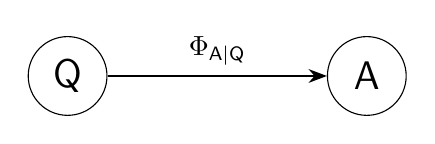
\begin{tikzpicture}[
        >=Stealth,
        node/.style={
            circle,
            draw,
            minimum size=1cm,
            font=\Large
        }
    ]
        \node[node] (Q) at (0,0) {$\mathsf{Q}$};
        \node[node] (A) at (3.8,0) {$\mathsf{A}$};
        \draw[->, thick] (Q) --
            node[midway,above] {$\Phi_{\mathsf{A}|\mathsf{Q}}$}
            (A);
    \end{tikzpicture}
    \caption{A channel network with compound input and output
    registers.}
    \label{fig:qbn2}
\end{figure}
\par
Its Q-factors are
\begin{enumerate}
    \item
    $\rho_{\mathsf{Q}}\in D(\mathcal{H}_{\mathsf{Q}})$;

    \item
    $\rho_{\mathsf{A}|\mathsf{Q}}
    \in
    \mathrm{Pos}(
        \mathcal{H}_{\mathsf{A}}
        \otimes
        \mathcal{H}_{\mathsf{Q}}
    )$, with
    \begin{equation}
        \mathrm{Tr}_{\mathcal{H}_{\mathsf{A}}}
        \left(
            \rho_{\mathsf{A}|\mathsf{Q}}
        \right)
        =
        \mathrm{Id}_{\mathcal{H}_{\mathsf{Q}}}.
    \end{equation}
\end{enumerate}

For the input register $\mathsf{Q}$, we use the indices
$i_{1},\dots,i_{n}$ and $j_{1},\dots,j_{n}$. For the output register
$\mathsf{A}$, we use $\alpha_{1},\dots,\alpha_{m}$ and
$\beta_{1},\dots,\beta_{m}$. The tensors are
\begin{enumerate}
    \item
    $\varrho_{\mathsf{Q}}
    \in
    \mathcal{H}_{\mathsf{Q}}
    \otimes
    \mathcal{H}_{\mathsf{Q}}^{*}$, with components
    $(\varrho_{\mathsf{Q}})
    ^{i_{1}\cdots i_{n}}{}_{j_{1}\cdots j_{n}}$;

    \item
    $\varrho_{\mathsf{A}|\mathsf{Q}}
    \in
    (\mathcal{H}_{\mathsf{A}}\otimes\mathcal{H}_{\mathsf{Q}})
    \otimes
    (\mathcal{H}_{\mathsf{A}}\otimes\mathcal{H}_{\mathsf{Q}})^{*}$,
    with components
    $(\varrho_{\mathsf{A}|\mathsf{Q}})
    ^{\alpha_{1}\cdots\alpha_{m}i_{1}\cdots i_{n}}
    {}_{\beta_{1}\cdots\beta_{m}j_{1}\cdots j_{n}}$;

    \item
    $\varrho_{\mathsf{A}}
    \in
    \mathcal{H}_{\mathsf{A}}
    \otimes
    \mathcal{H}_{\mathsf{A}}^{*}$, with components
    $(\varrho_{\mathsf{A}})
    ^{\alpha_{1}\cdots\alpha_{m}}
    {}_{\beta_{1}\cdots\beta_{m}}$.
\end{enumerate}
Let $\mathcal{B}_{\mathsf{Q}}$, $\mathcal{B}_{\mathsf{A}}$, and
$\mathcal{B}_{\mathsf{A}\mathsf{Q}}$ be the canonical bases of
$L(\mathcal{H}_{\mathsf{Q}})$,
$L(\mathcal{H}_{\mathsf{A}})$, and
$L(\mathcal{H}_{\mathsf{A}}\otimes\mathcal{H}_{\mathsf{Q}})$,
respectively. We set
\begin{equation}
    \begin{gathered}
    [\varrho_{\mathsf{Q}}]_{\mathcal{B}_{\mathsf{Q}}}
    =
    \rho_{\mathsf{Q}},
    \qquad
    [\varrho_{\mathsf{A}}]_{\mathcal{B}_{\mathsf{A}}}
    =
    \rho_{\mathsf{A}},\\
    [\varrho_{\mathsf{A}|\mathsf{Q}}]
    _{\mathcal{B}_{\mathsf{A}\mathsf{Q}}}
    =
    \rho_{\mathsf{A}|\mathsf{Q}}.
    \end{gathered}
\end{equation}
The component contraction is
\begin{equation}
    \begin{aligned}
    (\varrho_{\mathsf{A}})
    ^{\alpha_{1}\cdots\alpha_{m}}
    {}_{\beta_{1}\cdots\beta_{m}}
    &=
    (\varrho_{\mathsf{A}|\mathsf{Q}})
    ^{\alpha_{1}\cdots\alpha_{m}i_{1}\cdots i_{n}}
    {}_{\beta_{1}\cdots\beta_{m}j_{1}\cdots j_{n}}\\[-0.25em]
    &\quad\cdot
    (\varrho_{\mathsf{Q}})
    ^{i_{1}\cdots i_{n}}{}_{j_{1}\cdots j_{n}}.
    \end{aligned}
\end{equation}
Equivalently, if
\begin{equation}
    [\varsigma_{\mathsf{Q}}]_{\mathcal{B}_{\mathsf{Q}}}
    =
    \rho_{\mathsf{Q}}^{T},
\end{equation}
then the same operation takes the upper--lower form
\begin{equation}
    \begin{aligned}
    (\varrho_{\mathsf{A}})
    ^{\alpha_{1}\cdots\alpha_{m}}
    {}_{\beta_{1}\cdots\beta_{m}}
    &=
    (\varrho_{\mathsf{A}|\mathsf{Q}})
    ^{\alpha_{1}\cdots\alpha_{m}i_{1}\cdots i_{n}}
    {}_{\beta_{1}\cdots\beta_{m}j_{1}\cdots j_{n}}\\[-0.25em]
    &\quad\cdot
    (\varsigma_{\mathsf{Q}})
    ^{j_{1}\cdots j_{n}}{}_{i_{1}\cdots i_{n}}.
    \end{aligned}
\end{equation}
\subsection{Classical Bayesian networks in tensor form}
\label{subsec:classical-bn-tensor}

We now return to classical variables. As we saw in
Section~\ref{subsubsec:BN2}, products of classical Choi operators recover
the corresponding joint conditional operators once the factors have
been placed in a common operator space. Can the same calculation be
performed directly with tensors? Since classical probabilistic states
and conditional operators are diagonal, their factor product reduces to a pointwise product of their
nonzero components. This is the tensor form of the classical factor
product~\cite[Sec.~11.3.1]{Darwiche2008} and coincides with the purely
classical instance of the product of Q-factors
\cite[Sec.~3.1 and Def.~17]{DiGuardiaEhrhardFaggian2026}.
Throughout this subsection we use the explicit-output convention common in
programming implementations of Einsum
\cite[Sec.~2.8]{rocktai2018einsum}: every index displayed on the
left-hand side is a free output index, even if it occurs in several
factors on the right-hand side. An index is summed only when it is absent
from the output. Thus, indices repeated on both sides are multiplied
pointwise rather than contracted.

Consider first the two-node network in Fig.~\ref{fig:qbn3}.
\begin{figure}[ht]
    \centering
    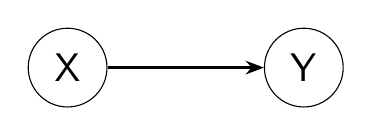
\begin{tikzpicture}[
        >=Stealth,
        node/.style={
            circle,
            draw,
            minimum size=1cm,
            font=\Large
        }
    ]
        \node[node] (Q1) at (0,0) {$\mathsf{X}$};
        \node[node] (Q2) at (3,0) {$\mathsf{Y}$};
        \draw[->, thick] (Q1) -- (Q2);
    \end{tikzpicture}
    \caption{A classical Bayesian network with two random variables.}
    \label{fig:qbn3}
\end{figure}

For the examples below, we consider binary-valued random variables. We
write
$\mathrm{Val}(\mathsf{X})=\{x^{t},x^{f}\}\cong\{0,1\}$,
where $x^{t}$ and $x^{f}$ denote true and false, respectively, and use
the same convention for every other variable. The joint alphabet of
$\mathsf{Y}$ and $\mathsf{X}$ is
$\mathrm{Val}(\mathsf{Y})\times\mathrm{Val}(\mathsf{X})$.
For each classical node $\mathsf{V}$, we write
$\mathcal{H}_{\mathsf{V}}=\mathbb{C}^{\mathrm{Val}(\mathsf{V})}$ for its
associated space, as in Sec.~\ref{sec:quantum-state}.

Let $\mathcal{B}_{\mathsf{X}}$ and
$\mathcal{B}_{\mathsf{Y}\mathsf{X}}$ denote the canonical bases of
$L(\mathcal{H}_{\mathsf{X}})$ and
$L(\mathcal{H}_{\mathsf{Y}}\otimes\mathcal{H}_{\mathsf{X}})$,
respectively. The root factor and the conditional factor are represented
by
\begin{enumerate}
    \item
    $\varrho_{\mathsf{X}}
    \in
    \mathcal{H}_{\mathsf{X}}\otimes\mathcal{H}_{\mathsf{X}}^{*}$,
    with components
    $(\varrho_{\mathsf{X}})^{x}{}_{x'}$ and
    $[\varrho_{\mathsf{X}}]_{\mathcal{B}_{\mathsf{X}}}
    =\rho_{\mathsf{X}}$;

    \item
    $\varrho_{\mathsf{Y}|\mathsf{X}}
    \in
    (\mathcal{H}_{\mathsf{Y}}\otimes\mathcal{H}_{\mathsf{X}})
    \otimes
    (\mathcal{H}_{\mathsf{Y}}\otimes\mathcal{H}_{\mathsf{X}})^{*}$,
    with components
    $(\varrho_{\mathsf{Y}|\mathsf{X}})
    ^{yx}{}_{y'x'}$ and
    $[\varrho_{\mathsf{Y}|\mathsf{X}}]
    _{\mathcal{B}_{\mathsf{Y}\mathsf{X}}}
    =\rho_{\mathsf{Y}|\mathsf{X}}$.
\end{enumerate}

Using this convention, the pointwise product of
$\varrho_{\mathsf{Y}|\mathsf{X}}$ and $\varrho_{\mathsf{X}}$ directly
defines $\varrho_{\mathsf{Y},\mathsf{X}}$. On the diagonal, this gives
\begin{equation}
    (\varrho_{\mathsf{Y},\mathsf{X}})
    ^{yx}{}_{yx}
    =
    (\varrho_{\mathsf{Y}|\mathsf{X}})
    ^{yx}{}_{yx}
    (\varrho_{\mathsf{X}})^{x}{}_{x}
    \label{eq:pointwise-factor}
\end{equation}
Here $y$ and $x$ are output indices, so they are not summed.

The full component expression is
\begin{equation}
    (\varrho_{\mathsf{Y},\mathsf{X}})
    ^{yx}{}_{y'x'}
    =
    (\varrho_{\mathsf{Y}|\mathsf{X}})
    ^{yx}{}_{y'x'}
    (\varrho_{\mathsf{X}})^{x}{}_{x'}.
\end{equation}
The factors on the right are diagonal, so all off-diagonal components
vanish and the nonzero entries are precisely the joint probabilities.
Consequently,
$[\varrho_{\mathsf{Y},\mathsf{X}}]
_{\mathcal{B}_{\mathsf{Y}\mathsf{X}}}
=\rho_{\mathsf{Y},\mathsf{X}}$.

\begin{example}
    Let
    \begin{equation}
        \begin{aligned}
        [\varrho_{\mathsf{X}}]_{\mathcal{B}_{\mathsf{X}}}
        &=
        \mathrm{diag}
        \begin{pmatrix}
            p_{\mathsf{X}}(x^{t})\\
            p_{\mathsf{X}}(x^{f})
        \end{pmatrix},\\
        [\varrho_{\mathsf{Y}|\mathsf{X}}]
        _{\mathcal{B}_{\mathsf{Y}\mathsf{X}}}
        &=
        \mathrm{diag}
        \begin{pmatrix}
            p_{\mathsf{Y}|\mathsf{X}}(y^{t}|x^{t})\\
            p_{\mathsf{Y}|\mathsf{X}}(y^{t}|x^{f})\\
            p_{\mathsf{Y}|\mathsf{X}}(y^{f}|x^{t})\\
            p_{\mathsf{Y}|\mathsf{X}}(y^{f}|x^{f})
        \end{pmatrix}.
        \end{aligned}
    \end{equation}
    Let $T$ be the diagonal type-$(2,2)$ tensor whose nonzero
    components are
    \begin{equation}
        T^{yx}{}_{yx}
        =
        (\varrho_{\mathsf{Y}|\mathsf{X}})
        ^{yx}{}_{yx}
        (\varrho_{\mathsf{X}})^{x}{}_{x},
    \end{equation}
    for $x,y\in\{0,1\}$, with no summation. Its components are
    \begin{align}
        T^{00}{}_{00}
        &=
        p_{\mathsf{Y}|\mathsf{X}}(y^{t}|x^{t})
        p_{\mathsf{X}}(x^{t})
        =
        p_{\mathsf{Y},\mathsf{X}}(y^{t},x^{t}),\\
        T^{01}{}_{01}
        &=
        p_{\mathsf{Y}|\mathsf{X}}(y^{t}|x^{f})
        p_{\mathsf{X}}(x^{f})
        =
        p_{\mathsf{Y},\mathsf{X}}(y^{t},x^{f}),\\
        T^{10}{}_{10}
        &=
        p_{\mathsf{Y}|\mathsf{X}}(y^{f}|x^{t})
        p_{\mathsf{X}}(x^{t})
        =
        p_{\mathsf{Y},\mathsf{X}}(y^{f},x^{t}),\\
        T^{11}{}_{11}
        &=
        p_{\mathsf{Y}|\mathsf{X}}(y^{f}|x^{f})
        p_{\mathsf{X}}(x^{f})
        =
        p_{\mathsf{Y},\mathsf{X}}(y^{f},x^{f}).
    \end{align}
    Hence $T=\varrho_{\mathsf{Y},\mathsf{X}}$.
\end{example}

We now consider the four-node network in Fig.~\ref{fig:qbn4}.
\begin{figure}[ht]
    \centering
    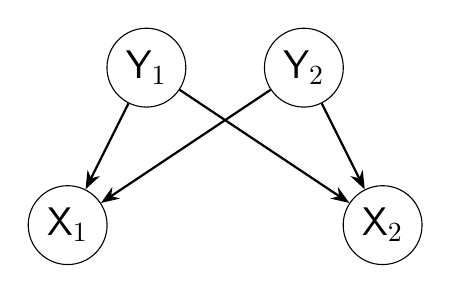
\begin{tikzpicture}[
        >=Stealth,
        node/.style={
            circle,
            draw,
            minimum size=1cm,
            font=\Large
        }
    ]
        \node[node] (Y1) at (1,2) {$\mathsf{Y}_{1}$};
        \node[node] (Y2) at (3,2) {$\mathsf{Y}_{2}$};
        \node[node] (X1) at (0,0) {$\mathsf{X}_{1}$};
        \node[node] (X2) at (4,0) {$\mathsf{X}_{2}$};

        \draw[->, thick] (Y1) -- (X1);
        \draw[->, thick] (Y1) -- (X2);
        \draw[->, thick] (Y2) -- (X2);
        \draw[->, thick] (Y2) -- (X1);
    \end{tikzpicture}
    \caption{A classical Bayesian network with four random variables.}
    \label{fig:qbn4}
\end{figure}

The root factors are represented by
$\varrho_{\mathsf{Y}_{r}}
\in
\mathcal{H}_{\mathsf{Y}_{r}}
\otimes
\mathcal{H}_{\mathsf{Y}_{r}}^{*}$, with components
$(\varrho_{\mathsf{Y}_{r}})^{y_{r}}{}_{y'_{r}}$ for
$r\in\{1,2\}$. For each $r\in\{1,2\}$, the conditional factor is
\begin{equation*}
    \varrho_{\mathsf{X}_{r}|\mathsf{Y}_{1},\mathsf{Y}_{2}}
    \in{}
    (\mathcal{H}_{\mathsf{X}_{r}}
    \otimes\mathcal{H}_{\mathsf{Y}_{1}}
    \otimes\mathcal{H}_{\mathsf{Y}_{2}})
    \otimes
    (\mathcal{H}_{\mathsf{X}_{r}}
    \otimes\mathcal{H}_{\mathsf{Y}_{1}}
    \otimes\mathcal{H}_{\mathsf{Y}_{2}})^{*},
\end{equation*}
with components
\[
    (\varrho_{\mathsf{X}_{r}|\mathsf{Y}_{1},\mathsf{Y}_{2}})
    ^{x_{r}y_{1}y_{2}}{}_{x'_{r}y'_{1}y'_{2}}.
\]
Its classical alphabet is
$\mathrm{Val}(\mathsf{X}_{r})
\times\mathrm{Val}(\mathsf{Y}_{1})
\times\mathrm{Val}(\mathsf{Y}_{2})$.

The graph implies
$\mathsf{X}_{1}\perp\mathsf{X}_{2}
\mid(\mathsf{Y}_{1},\mathsf{Y}_{2})$, while the two root variables
$\mathsf{Y}_{1}$ and $\mathsf{Y}_{2}$ are independent. The
Bayesian-network factorization therefore gives the following diagonal
component identities~\cite[Sec.~11.2.3, Eq.~(11.3)]{Darwiche2008}.
Every displayed index is an output index, so no summation is performed.
To simplify the notation, let
\begin{equation}
    \mathbf{X}=(\mathsf{X}_{1},\mathsf{X}_{2}),
    \qquad
    \mathbf{Y}=(\mathsf{Y}_{1},\mathsf{Y}_{2}),
\end{equation}
and write
\begin{equation}
    \mathbf{x}=(x_{1},x_{2}),
    \qquad
    \mathbf{y}=(y_{1},y_{2}).
\end{equation}
The bold indices abbreviate these ordered pairs. Their individual entries
remain free, so this notation does not introduce any summation.
\begin{equation}
    (\varrho_{\mathbf{X}|\mathbf{Y}})
    ^{\mathbf{x}\mathbf{y}}{}_{\mathbf{x}\mathbf{y}}
    =
    (\varrho_{\mathsf{X}_{1}|\mathbf{Y}})
    ^{x_{1}\mathbf{y}}{}_{x_{1}\mathbf{y}}
    (\varrho_{\mathsf{X}_{2}|\mathbf{Y}})
    ^{x_{2}\mathbf{y}}{}_{x_{2}\mathbf{y}}.
\end{equation}
\begin{equation}
    \begin{aligned}
    (\varrho_{\mathbf{X},\mathsf{Y}_{1}|\mathsf{Y}_{2}})
    ^{\mathbf{x}\mathbf{y}}{}_{\mathbf{x}\mathbf{y}}
    &=
    (\varrho_{\mathsf{X}_{1}|\mathbf{Y}})
    ^{x_{1}\mathbf{y}}{}_{x_{1}\mathbf{y}}
    (\varrho_{\mathsf{X}_{2}|\mathbf{Y}})
    ^{x_{2}\mathbf{y}}{}_{x_{2}\mathbf{y}}\\
    &\quad\cdot
    (\varrho_{\mathsf{Y}_{1}})^{y_{1}}{}_{y_{1}}.
    \end{aligned}
\end{equation}
\begin{equation}
    \begin{aligned}
    (\varrho_{\mathbf{X},\mathbf{Y}})
    ^{\mathbf{x}\mathbf{y}}{}_{\mathbf{x}\mathbf{y}}
    &=
    (\varrho_{\mathsf{X}_{1}|\mathbf{Y}})
    ^{x_{1}\mathbf{y}}{}_{x_{1}\mathbf{y}}
    (\varrho_{\mathsf{X}_{2}|\mathbf{Y}})
    ^{x_{2}\mathbf{y}}{}_{x_{2}\mathbf{y}}\\
    &\quad\cdot
    (\varrho_{\mathsf{Y}_{1}})^{y_{1}}{}_{y_{1}}
    (\varrho_{\mathsf{Y}_{2}})^{y_{2}}{}_{y_{2}}.
    \end{aligned}
\end{equation}
These identities illustrate one of the main advantages of the tensor
formulation. Unlike the matrix formalism in
Section~\ref{subsubsec:BN2}, there is no need to construct the full
lifted matrices before multiplying the factors. The indices determine
the variables shared by the factors, and a factor that does not contain
one of the output indices is simply multiplied across all values of that
index. The joint probabilities are therefore obtained directly from the
pointwise product of the corresponding components.

\subsection{Hybrid classical--quantum networks}

\subsubsection{Hybrid operators}

We now consider networks containing both classical and quantum nodes. Their
local factors are operators on tensor products of classical and quantum
register spaces. We place all classical registers before all quantum
registers and use the same order for their component indices. When this
differs from the output--input order of Sec.~\ref{subsubsec:choi-isomorphism},
we use the canonical permutation of the tensor factors. All transposes are
taken in the chosen orthonormal bases.

Let $\mathsf{X}$ be a classical node with alphabet $\Sigma$. Its associated
space is
$\mathcal{H}_{\mathsf{X}}=\mathbb{C}^{\Sigma}$, with standard basis
$\{\ket{x}:x\in\Sigma\}$ indexed by the possible values of $\mathsf{X}$.
Let $\mathsf{Q}$ be a quantum node with associated space
$\mathcal{H}_{\mathsf{Q}}$. The composite space is
\begin{equation}
    \mathcal{H}_{\mathsf{X}\mathsf{Q}}
    =
    \mathcal{H}_{\mathsf{X}}
    \otimes
    \mathcal{H}_{\mathsf{Q}}.
\end{equation}

\begin{definition}
    \label{def:hybrid-operator}
    A \emph{hybrid operator} on
    $\mathcal{H}_{\mathsf{X}\mathsf{Q}}$ is an operator of the form
    \begin{equation}
        \sigma_{\mathsf{X}\mathsf{Q}}
        =
        \sum_{x\in\Sigma}
        \ket{x}\!\bra{x}_{\mathsf{X}}
        \otimes
        M_x^{\mathsf{Q}},
    \end{equation}
    where $\{M_x^{\mathsf{Q}}:x\in\Sigma\}$ is a family of operators
    on $\mathcal{H}_{\mathsf{Q}}$, indexed by the values of
    $\mathsf{X}$~\cite[Def.~III.10]{LeiferSpekkens2013}.

    When $\mathsf{X}$ is a parent of $\mathsf{Q}$, the corresponding
    conditional factor has the form
    \begin{equation}
        \sigma_{\mathsf{Q}|\mathsf{X}}
        =
        \sum_{x\in\Sigma}
        \ket{x}\!\bra{x}_{\mathsf{X}}
        \otimes
        \rho_x^{\mathsf{Q}},
    \end{equation}
    where $\rho_x^{\mathsf{Q}}\in D(\mathcal{H}_{\mathsf{Q}})$ for every
    $x\in\Sigma$. It is positive and conditionally normalized:
    \begin{equation}
        \mathrm{Tr}_{\mathcal{H}_{\mathsf{Q}}}
        \left(\sigma_{\mathsf{Q}|\mathsf{X}}\right)
        =
        \mathrm{Id}_{\mathcal{H}_{\mathsf{X}}}.
    \end{equation}
    When $\mathsf{Q}$ is a parent of $\mathsf{X}$, a POVM
    $\{P_x^{\mathsf{Q}}:x\in\Sigma\}$ defines the conditional factor
    \begin{equation}
        \sigma_{\mathsf{X}|\mathsf{Q}}
        =
        \sum_{x\in\Sigma}
        \ket{x}\!\bra{x}_{\mathsf{X}}
        \otimes
        \left(P_x^{\mathsf{Q}}\right)^{T},
    \end{equation}
    which is positive and satisfies
    \begin{equation}
        \mathrm{Tr}_{\mathcal{H}_{\mathsf{X}}}
        \left(\sigma_{\mathsf{X}|\mathsf{Q}}\right)
        =
        \mathrm{Id}_{\mathcal{H}_{\mathsf{Q}}}.
    \end{equation}
\end{definition}

When the components $M_x^{\mathsf{Q}}$ are positive, this block-diagonal
operator encodes the Q-factor
$x\mapsto M_x^{\mathsf{Q}}$~\cite[Def.~13]{DiGuardiaEhrhardFaggian2026}.
The transpose in $\sigma_{\mathsf{X}|\mathsf{Q}}$ follows from the Choi convention of
Sec.~\ref{subsubsec:choi-isomorphism}: the measurement channel
$A\mapsto\sum_x\mathrm{Tr}(P_x^{\mathsf{Q}}A)
\ket{x}\!\bra{x}_{\mathsf{X}}$ has this Choi operator.

\subsubsection{A preparation--measurement network}

Consider the hybrid network
\begin{figure}[ht]
    \centering
    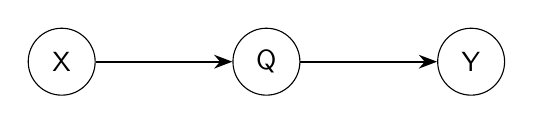
\begin{tikzpicture}[
        >=Stealth,
        node/.style={
            circle,
            draw,
            minimum size=0.85cm,
            font=\normalsize
        }
    ]
        \node[node] (X) at (0,0) {$\mathsf{X}$};
        \node[node] (Q) at (2.6,0) {$\mathsf{Q}$};
        \node[node] (Y) at (5.2,0) {$\mathsf{Y}$};
        \draw[->, thick] (X) -- (Q);
        \draw[->, thick] (Q) -- (Y);
    \end{tikzpicture}
    \caption{A preparation--measurement network with classical nodes
    $\mathsf{X}$ and $\mathsf{Y}$ and quantum node $\mathsf{Q}$.}
    \label{fig:hybrid-network}
\end{figure}

Let $\Sigma$ and $\Gamma$ be the alphabets of $\mathsf{X}$ and
$\mathsf{Y}$, respectively. The associated Q-factors are
\begin{enumerate}
    \item the classical factor associated with the node
    $\mathsf{X}$ is $\rho_{\mathsf{X}}$;

    \item the hybrid factor associated with the node
    $\mathsf{Q}$ is $\rho_{\mathsf{Q}|\mathsf{X}}$;

    \item the hybrid factor associated with the node
    $\mathsf{Y}$ is $\rho_{\mathsf{Y}|\mathsf{Q}}$.
\end{enumerate}
Here, $p_{\mathsf{X}}$ is the distribution encoded by
$\rho_{\mathsf{X}}$, the states
$\{\rho_x^{\mathsf{Q}}:x\in\Sigma\}$ define the preparation factor, and
the POVM $\{P_y^{\mathsf{Q}}:y\in\Gamma\}$ defines the measurement factor
as in Definition~\ref{def:hybrid-operator}.

We now use the operator-to-tensor representation described in
Sec.~\ref{subsec:tensors-contractions}. Choose a fixed orthonormal basis
$\{\ket{q}:q\in\Lambda\}$ of
$\mathcal{H}_{\mathsf{Q}}$. Let $\mathcal{B}_{\mathsf{X}}$,
$\mathcal{B}_{\mathsf{X}\mathsf{Q}}$, and
$\mathcal{B}_{\mathsf{Y}\mathsf{Q}}$ denote the canonical bases of
$L(\mathcal{H}_{\mathsf{X}})$,
$L(\mathcal{H}_{\mathsf{X}}\otimes\mathcal{H}_{\mathsf{Q}})$, and
$L(\mathcal{H}_{\mathsf{Y}}\otimes\mathcal{H}_{\mathsf{Q}})$,
respectively. Quantum indices are contracted according to the coordinate
convention of Sec.~\ref{subsubsec:pqf}. For classical indices, we use the
explicit-output convention of Sec.~\ref{subsec:classical-bn-tensor},
illustrated in Eq.~\ref{eq:pointwise-factor}: indices displayed on the
left-hand side remain free and are multiplied pointwise. The tensors
corresponding to the three Q-factors are
\begin{enumerate}
    \item
    $\varrho_{\mathsf{X}}
    \in
    \mathcal{H}_{\mathsf{X}}
    \otimes
    \mathcal{H}_{\mathsf{X}}^{*}$,
    with components
    $(\varrho_{\mathsf{X}})^{x}{}_{x'}$ and
    \begin{equation}
        [\varrho_{\mathsf{X}}]_{\mathcal{B}_{\mathsf{X}}}
        =
        \rho_{\mathsf{X}};
    \end{equation}

    \item
    $\varrho_{\mathsf{Q}|\mathsf{X}}
    \in
    (\mathcal{H}_{\mathsf{X}}\otimes\mathcal{H}_{\mathsf{Q}})
    \otimes
    (\mathcal{H}_{\mathsf{X}}\otimes\mathcal{H}_{\mathsf{Q}})^{*}$,
    with components
    $(\varrho_{\mathsf{Q}|\mathsf{X}})^{xq}{}_{x'q'}$ and
    \begin{equation}
        [\varrho_{\mathsf{Q}|\mathsf{X}}]
        _{\mathcal{B}_{\mathsf{X}\mathsf{Q}}}
        =
        \rho_{\mathsf{Q}|\mathsf{X}};
    \end{equation}

    \item
    $\varrho_{\mathsf{Y}|\mathsf{Q}}
    \in
    (\mathcal{H}_{\mathsf{Y}}\otimes\mathcal{H}_{\mathsf{Q}})
    \otimes
    (\mathcal{H}_{\mathsf{Y}}\otimes\mathcal{H}_{\mathsf{Q}})^{*}$,
    with components
    $(\varrho_{\mathsf{Y}|\mathsf{Q}})^{yq}{}_{y'q'}$ and
    \begin{equation}
        [\varrho_{\mathsf{Y}|\mathsf{Q}}]
        _{\mathcal{B}_{\mathsf{Y}\mathsf{Q}}}
        =
        \rho_{\mathsf{Y}|\mathsf{Q}}.
    \end{equation}
\end{enumerate}

Combining the three Q-factors using this component convention gives a
tensor on the two classical nodes $\mathsf{X}$ and $\mathsf{Y}$:
\begin{equation}
    (\varrho_{\mathsf{X},\mathsf{Y}})^{xy}{}_{x'y'}=
    (\varrho_{\mathsf{X}})^{x}{}_{x'}
    (\varrho_{\mathsf{Q}|\mathsf{X}})^{xq}{}_{x'q'}(\varrho_{\mathsf{Y}|\mathsf{Q}})^{yq}{}_{y'q'}.
\end{equation}
Because the measurement is modeled as destructive,
$\varrho_{\mathsf{Y}|\mathsf{Q}}$ has quantum input indices but no quantum
output indices. Its indices $q$ and $q'$ are contracted with those
introduced by $\varrho_{\mathsf{Q}|\mathsf{X}}$. On the diagonal,
\begin{equation}
    \begin{aligned}
    (\varrho_{\mathsf{X},\mathsf{Y}})^{xy}{}_{xy}
    &=
    p_{\mathsf{X}}(x)
    \sum_{q,q'}
    \left(\rho_x^{\mathsf{Q}}\right)^{q}{}_{q'}
    \left(\left(P_y^{\mathsf{Q}}\right)^{T}\right)^{q}{}_{q'}\\
    &=
    p_{\mathsf{X}}(x)
    \mathrm{Tr}\left(
        P_y^{\mathsf{Q}}\rho_x^{\mathsf{Q}}
    \right).
    \end{aligned}
\end{equation}
All off-diagonal classical components vanish. Since
$\sum_yP_y^{\mathsf{Q}}=\mathrm{Id}_{\mathcal{H}_{\mathsf{Q}}}$, these
components form a normalized joint distribution on
$(\mathsf{X},\mathsf{Y})$.

\section{Conclusion and outlook}

We began with the question of whether the local factors associated with
classical and quantum nodes could be described within the same operator
formalism. Encoding finite probability distributions as diagonal density
operators provides such a description. A conditional distribution then
determines a positive operator that is exactly the Choi operator of the
quantum channel induced by the corresponding stochastic map. Classical
conditional factors therefore appear as a special case of the channel
factors used for quantum nodes.

In fixed bases, the tensor representation makes the action and composition
of these factors more direct. The transpose, operator multiplication, and
partial trace in the usual Choi action are collected into a contraction over
the input indices, while the intermediate register remains explicit in a
composition of channels. For diagonal operators, multiplication reduces to
the pointwise product of probability factors. In the hybrid example, the
contraction between a preparation and a destructive measurement removes the
quantum indices and leaves a factor on the classical registers.

We have focused on the representation and combination of local factors,
rather than on a complete theory of inference for quantum Bayesian networks.
The component formulation depends on the chosen orthonormal bases and on a
fixed ordering of the registers. A natural continuation would be to extend
these rules to general hybrid directed acyclic graphs and study how they
interact with marginalization, conditioning, and inference. 

\begin{acknowledgments}
I would like to thank Claudia Faggian for her supervision, guidance, and
valuable discussions throughout this work, and Gabriele Tedeschi for
helpful discussions and feedback. I also acknowledge the use of OpenAI
Codex, using the GPT-5.6 Sol model, to assist with the organization and
presentation of the manuscript, the formulation of parts of the exposition,
checking citations, reviewing mathematical derivations developed by the
author, and resolving selected \LaTeX{} layout issues. No AI system,
including Codex, was used to originate the research questions, mathematical
framework, results, or original derivations presented in this work. These
were developed by the author under Claudia Faggian's supervision. All
mathematical arguments and the final content of the manuscript remain the
responsibility of the author.
\end{acknowledgments}

\bibliographystyle{apsrev4-2}
\bibliography{references}

\end{document}

